\part{Reconnaissance (TA0043)}
\chapter{Introduction}
\section{Enumeration Principles}

Enumeration is a widely used term in cyber security. It stands for information
gathering using active (scans) and passive (use of third-party providers)
methods. It is important to note that OSINT is an independent procedure and
should be performed separately from enumeration because {\emph OSINT is based
exclusively on passive information gathering} and does not involve active
enumeration of the given target. Enumeration is a loop in which we repeatedly
gather information based on what data we have or have already discovered.

Information can be gathered from domains, IP addresses, accessible services,
and many other sources.

Once we have identified targets in our client's infrastructure, we need to
examine the individual services and protocols. In most cases, these are
services that enable communication between customers, the infrastructure, the
administration, and the employees.

If we imagine that we have been hired to investigate the IT security of a
company, we will start to develop a general understanding of the company's
functionality. For example, we need to understand how the company is
structured, what services and third-party vendors it uses, what security
measures may be in place, and more. This is where this stage can be a bit
misunderstood because most people focus on the obvious and try to force their
way into the company's systems instead of understanding how the infrastructure
is set up and what technical aspects and services are necessary to be able to
offer a specific service.

An example of such a wrong approach could be that after finding authentication
services like SSH, RDP, WinRM, and the like, we try to brute-force with
common/weak passwords and usernames. Unfortunately, brute-forcing is a noisy
method and can easily lead to blacklisting, making further testing impossible.
Primarily, this can happen if we do not know about the company's defensive
security measures and its infrastructure. Some may smile at this approach, but
experience has shown that far too many testers take this type of approach.

{\bf Our goal is not to get at the systems but to find all the ways to get there.}

The enumeration principles are based on some questions that will facilitate all
our investigations in any conceivable situation. In most cases, the main focus
of many penetration testers is on what they can see and not on what they cannot
see. However, even what we cannot see is relevant to us and may well be of
great importance. The difference here is that we start to see the components
and aspects that are not visible at first glance with our experience.
\begin{itemize}
        \item What can we see?
        \item What reasons can we have for seeing it?
        \item What image does what we see create for us?
        \item What do we gain from it?
        \item How can we use it?
        \item What can we not see?
        \item What reasons can there be that we do not see?
        \item What image results for us from what we do not see?
\end{itemize}

An important aspect that must not be confused here is that there are always
exceptions to the rules. The principles, however, do not change. Another
advantage of these principles is that we can see from the practical tasks that
we do not lack penetration testing abilities but technical understanding when
we suddenly do not know how to proceed because our core task is not to exploit
the machines but to find how they can be exploited.

Principles:
\begin{enumerate}
    \item There is more than meets the eye. Consider all points of view.
    \item Distinguish between what we see and what we do not see.
    \item There are always ways to gain more information. Understand the target.
\end{enumerate}


\section{ Enumeration Methodology}


Complex processes must have a standardized methodology that helps us keep our
bearings and avoid omitting any aspects by mistake. Especially with the variety
of cases that the target systems can offer us, it is almost unpredictable how
our approach should be designed. Therefore, most penetration testers follow
their habits and the steps they feel most comfortable and familiar with.
However, this is not a standardized methodology but rather an experience-based
approach.

We know that penetration testing, and therefore enumeration, is a dynamic
process. Consequently, we have developed a static enumeration methodology for
external and internal penetration tests that includes free dynamics and allows
for a wide range of changes and adaptations to the given environment. This
methodology is nested in 6 layers and represents, metaphorically speaking,
boundaries that we try to pass with the enumeration process. The whole
enumeration process is divided into three different levels:
\begin{itemize}
    \item Infrastructure-based enumeration 	
    \item Host-based enumeration 	
    \item OS-based enumeration
\end{itemize}



\begin{figure}
    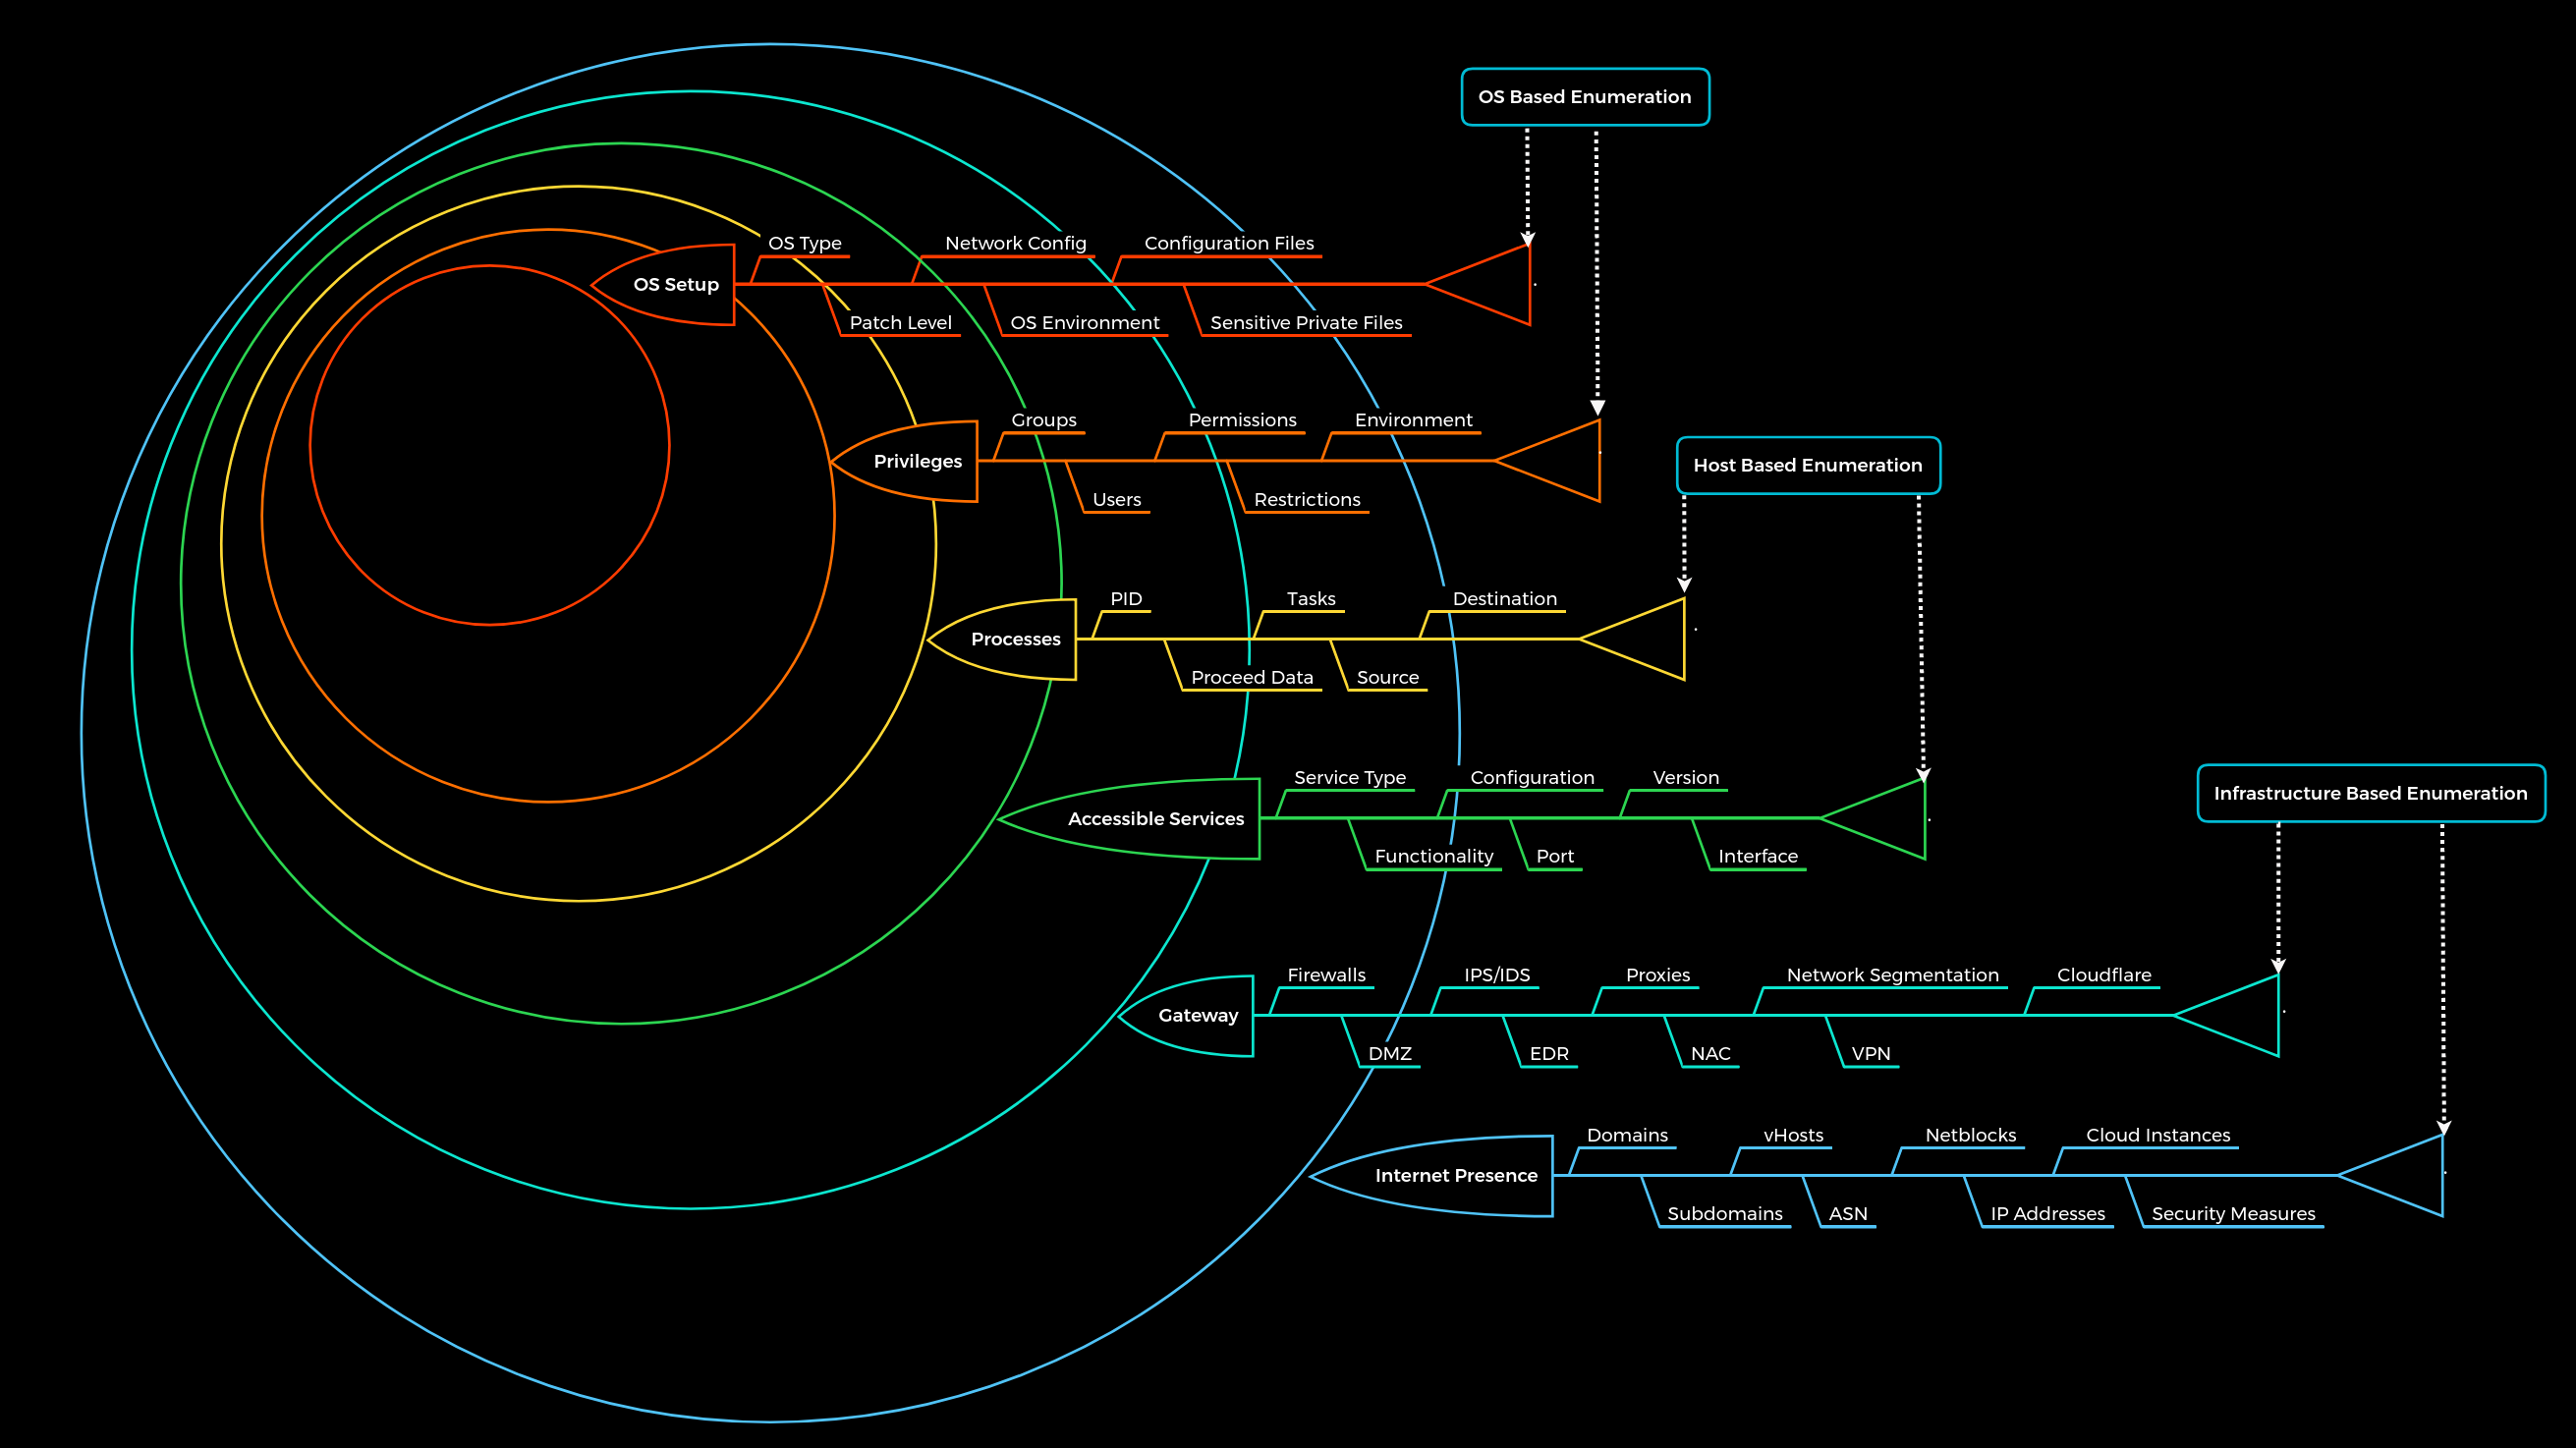
\includegraphics[angle=90,origin=c,width=\linewidth]{recon/intro/images/enum-method.png}
  \caption{Enumeration methodology}
  \label{fig:pentest-process-enum-method}
\end{figure}

Consider these lines as some kind of obstacle, like a wall, for example. What
we do here is look around to find out where the entrance is, or the gap we can
fit through, or climb over to get closer to our goal. Theoretically, it is also
possible to go through the wall headfirst, but very often, it happens that the
spot we have smashed the gap with a lot of effort and time with force does not
bring us much because there is no entry at this point of the wall to pass on to
the next wall.

\begin{itemize}
\item {\bf Internet Presence}: The first layer we have to pass is the
    "Internet Presence" layer, where we focus on finding the targets we can
    investigate. If the scope in the contract allows us to look for additional
    hosts, this layer is even more critical than for fixed targets only. In
    this layer, we use different techniques to find domains, subdomains,
    netblocks, and many other components and information that present the
    presence of the company and its infrastructure on the Internet.

    Identification of internet presence and
    externally accessible infrastructure (Domains, Subdomains, vHosts, ASN,
    Netblocks, IP Addresses, Cloud Instances, Security Measures)
    {\bf The goal of this layer is to identify all possible target systems and
    interfaces that can be tested.}
\item {\bf Gateway}:  	Identify the possible security measures to protect the
    company's external and internal infrastructure (Firewalls, DMZ, IPS/IDS,
    EDR, Proxies, NAC, Network Segmentation, VPN, Cloudflare)
    {\bf The goal is to understand what we are dealing with and what we have to
    watch out for.}
\item {\bf Accessible Services} 	Identify accessible interfaces and services
    that are hosted externally or internally (Service Type, Functionality,
    Configuration, Port, Version, Interface).
    {\bf This layer aims to understand the reason and functionality of the
        target system and gain the necessary knowledge to communicate with it
    and exploit it for our purposes effectively.}
\item {\bf Processes} 	Every time a command or function is executed, data is
    processed, whether entered by the user or generated by the system. This
    starts a process that has to perform specific tasks, and such tasks have at
    least one source and one target.
    {\bf The goal here is to understand these factors and identify the
    dependencies between them.} Identify the internal processes, sources, and
    destinations associated with the services (PID, Proceed Data, Tasks,
    Source, Destination)
\item {\bf Privileges} 	Each service runs through a specific user in a
    particular group with permissions and privileges defined by the
    administrator or the system. These privileges often provide us with
    functions that administrators overlook. This often happens in Active
    Directory infrastructures and many other case-specific administration
    environments and servers where users are responsible for multiple
    administration areas.
    {\bf It is crucial to identify these and understand what is and is not possible with
these privileges.}Identification of the internal permissions and
    privileges to the accessible services (Groups, Users, Permissions,
    Restrictions, Environment)
\item {\bf OS Setup} Here we collect information about the actual operating
    system and its setup using internal access. This gives us a good overview
    of the internal security of the systems and reflects the skills and
    capabilities of the company's administrative teams.
    {\bf The goal here is to see how the administrators manage the systems and what
sensitive internal information we can glean from them.}	Identification of the
internal components and systemsasetup (OS Type, Patch Level, Network config, OS
Environment, Configuration files, sensitive private files \ldots)
\end{itemize}

We can finally imagine the entire penetration test in the form of a labyrinth
where we have to identify the gaps and find the way to get us inside as quickly
and effectively as possible. This type of labyrinth may look something like
this:

\begin{figure}
    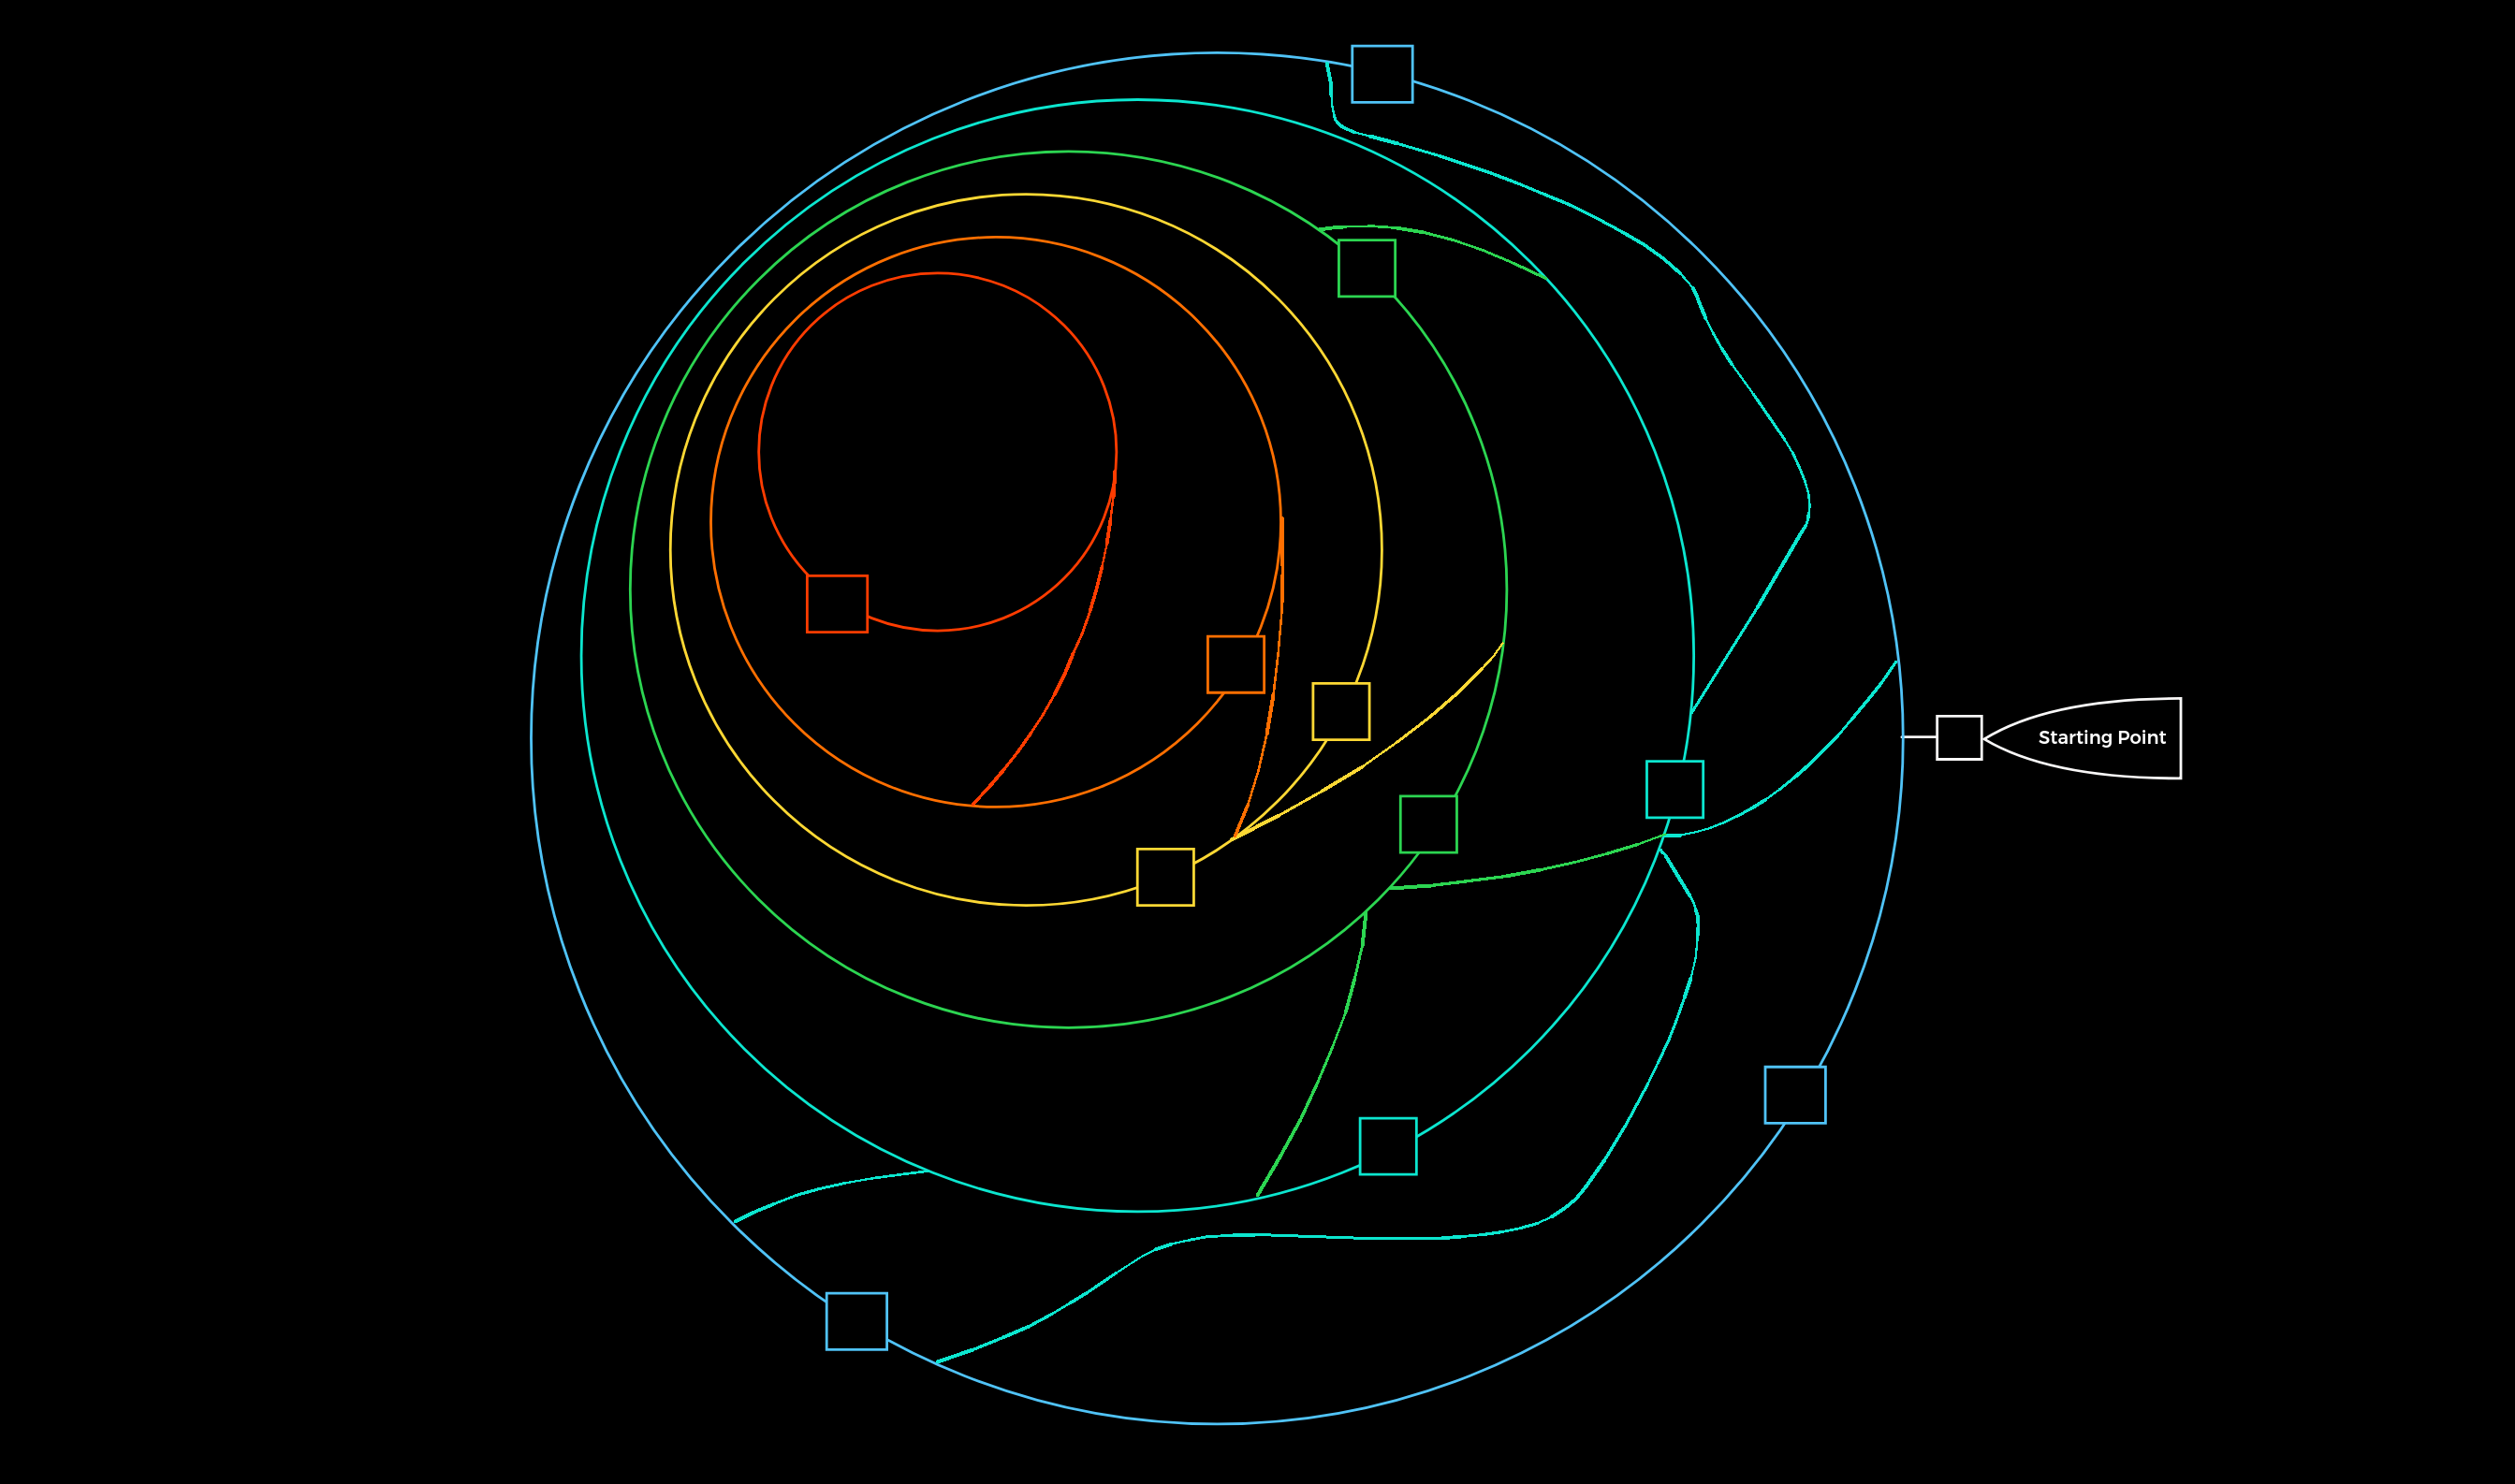
\includegraphics[angle=90,origin=c,width=\linewidth]{recon/intro/images/pentest-labyrinth.png}
  \caption{Pentest labyrinth}
  \label{fig:pentest-pentest-labyrinth}
\end{figure}

As we have probably already noticed, we can see that we will encounter one gap
and very likely several. The interesting and very common fact is that not all
the gaps we find can lead us inside. All penetration tests are limited in time,
but we should always keep in mind that one belief that there is nearly always a
way in. Even after a four-week penetration test, we cannot say 100\% that there
are no more vulnerabilities. Someone who has been studying the company for
months and analyzing them will most likely have a much greater understanding of
the applications and structure than we were able to gain within the few weeks
we spent on the asessment. 

\section{Enumeration Methodology in Practice}

A methodology summarizes all systematic procedures in obtaining knowledge
within the bounds of a given objective. It is important to note that a
methodology is not a step-by-step guide but, as the definition implies, a
summary of systematic procedures. In our case, the enumeration methodology is
the systematic approach to explore a given target.

How the individual components are identified and information obtained in this
methodology is a dynamic and growing aspect that is constantly changing and can
therefore differ. An excellent example of this is using information-gathering
tools from web servers. There are countless different tools for this, and each
of them has a specific focus and therefore delivers individual results that
differ from other applications. The goal, however, is the same. Thus, the
collection of tools and commands is not part of the actual methodology but
rather a cheat sheet that we can refer to using the commands and tools listed
in given cases.


\chapter{Internet presence}


\section{What to look for}
\begin{tabularx}{\linewidth}{|l|X|}
\hline
Data Point &	Description\\
\hline
IP Space &	Valid \gls{ASN}, netblocks in use for the public-facing infrastructure,
cloud presence and the hosting providers, DNS record entries, \ldots\\
\hline
Domain Information & 	Based on IP data, DNS, and site registrations. Who
administers the domain? Are there any subdomains tied ? Are there
any publicly accessible domain services present? (Mailservers, DNS, Websites,
VPN portals, etc.) Can we determine what kind of defenses are in place? (SIEM,
AV, IPS/IDS in use, \ldots)\\
\hline
Schema Format &	Can we discover email accounts, AD
usernames, and even password policies? Anything that will give information that
can be used to build a valid username list to test external-facing services for
password spraying, credential stuffing, brute forcing, \ldots.\\
\hline
Data Disclosures &	looking fublicly accessible files ( .pdf, .ppt, .docx,
.xlsx, \ldots ) for any information that helps shed light on the target. For
example, any published files that contain intranet site listings, user
metadata, shares, or other critical software or hardware in the environment
(credentials pushed to a public GitHub repo, the internal AD username format in
the metadata of a PDF, for example. )\\
\hline
Breach Data &	Any publicly released usernames, passwords, or other critical
information that can help  gain a foothold.\\
\hline
\end{tabularx}

\section{Where looking ?}

\begin{tabularx}{\linewidth}{|l|X|}
\hline
Resource & 	Examples \\
\hline
\hline
Social Media &	Searching Linkedin, Twitter, Facebook, your region's major
social media sites, news articles, and any relevant info you can find about the
organization.\\
\hline
Public-Facing Company Websites & 	Often, the public website for a corporation
will have relevant info embedded. News articles, embedded documents, and the
"About Us" and "Contact Us" pages can also be gold mines.\\
\hline
Cloud \& Dev Storage Spaces &	\href{https://github.com/}{GitHub}, \href{https://grayhatwarfare.com/}{AWS S3 buckets \& Azure Blog storage
containers}, \href{https://www.exploit-db.com/google-hacking-database}{Google
searches using "Dorks"}\\
\hline
Breach Data Sources &	\href{https://haveibeenpwned.com/}{HaveIBeenPwned}to determine if any corporate email
accounts appear in public breach data, \href{https://www.dehashed.com/}{Dehashed} to search for corporate emails
with cleartext passwords or hashes we can try to crack offline. We can then try
these passwords against any exposed login portals (Citrix, RDS, OWA, 0365, VPN,
VMware Horizon, custom applications, etc.) that may use AD authentication.\\
\hline
\end{tabularx}

\section{Domain information}

Domain information is a core component of any penetration test, and it is not
just about the subdomains but about the entire presence on the Internet.
Therefore, we gather information and try to understand the company's
functionality and which technologies and structures are necessary for services
to be offered successfully and efficiently.

This type of information is gathered passively without direct and active scans.
In other words, we remain hidden and navigate as "customers" or "visitors" to
avoid direct connections to the company that could expose us. The OSINT
relevant sections are only a tiny part of how in-depth OSINT goes and describe
only a few of the many ways to obtain information in this way.

However, when passively gathering information, we can use third-party services
to understand the company better. However, the first thing we should do is
scrutinize the company's main website. Then, we should read through the texts,
keeping in mind what technologies and structures are needed for these
services.

For example, many IT companies offer app development, IoT, hosting, data
science, and IT security services, depending on their industry. If we encounter
a service that we have had little to do with before, it makes sense and is
necessary to get to grips with it and find out what activities it consists of
and what opportunities are available. Those services also give us a good
overview of how the company can be structured.

For example, this part is the combination between the {\emph first principle}
and the '\emph second principle} of enumeration. We pay attention to what
{\emph we see}  and {\emph we do not see}. We see the services but not their
functionality. However, services are bound to certain technical aspects
necessary to provide a service. Therefore, we take the developer's view and
look at the whole thing from their point of view. This point of view allows us
to gain many technical insights into the functionality.

Once we have a basic understanding of the company and its services, we can get
a first impression of its presence on the Internet. Let us assume that a
medium-sized company has hired us to test their entire infrastructure from a
black-box perspective. This means we have only received a scope of targets and
must obtain all further information ourselves.

\subsection{SSL certificates enumeration}

The first point of presence on the Internet may be the {\bf SSL certificate}
from the company's main website that we can examine. Often, such a certificate
includes more than just a subdomain, and this means that the certificate is
used for several domains, and these are most likely still active.

Another source to find more subdomains is \href{https://crt.sh/}{crt.sh}. This
source is
\href{https://en.wikipedia.org/wiki/Certificate_Transparency}{Certificate
Transparency} logs. Certificate Transparency is a process that is intended to
enable the verification of issued digital certificates for encrypted Internet
connections. The standard (\href{https://tools.ietf.org/html/rfc6962}{RFC
6962}) provides for the logging of all digital certificates issued by a
certificate authority in audit-proof logs. This is intended to enable the
detection of false or maliciously issued certificates for a domain. SSL
certificate providers like Let's Encrypt share this with the web interface
crt.sh, which stores the new entries in the database to be accessed later.

\begin{verbatim}
curl -s https://crt.sh/\?q\=inlanefreight.com\&output\=json | jq .

curl -s https://crt.sh/\?q\=inlanefreight.com\&output\=json \
    | jq . \
    | grep name \
    | cut -d":" -f2 \
    | grep -v "CN=" \
    | cut -d'"' -f2 \
    | awk '{gsub(/\\n/,"\n");}1;' \
    | sort -u
\end{verbatim}

\input{recon/internet/IP}
\section{Cloud resources}

The use of cloud, such as AWS, GCP, Azure, and others, is now one of the
essential components for many companies nowadays. After all, all companies want
to be able to do their work from anywhere, so they need a central point for all
management. This is why services from Amazon (AWS), Google (GCP), and Microsoft
(Azure) are ideal for this purpose.

Even though cloud providers secure their infrastructure centrally, this does
not mean that companies are free from vulnerabilities. The configurations made
by the administrators may nevertheless make the company's cloud resources
vulnerable. This often starts with the S3 buckets (AWS), blobs (Azure), cloud
storage (GCP), which can be accessed without authentication if configured
incorrectly.

Often cloud storage is added to the DNS list when used for administrative
purposes by other employees. This step makes it much easier for the employees
to reach and manage them.

However, there are many different ways to find such cloud storage. 

\subsection{Google Dorks}

One of the easiest and most used is Google search combined with Google Dorks.
For example, we can use the
\href{https://www.exploit-db.com/google-hacking-database}{Google Dorks}
\verb+inurl:+ and \verb+intext:+ to narrow our search to specific terms.

\begin{verbatim}
intext:COMPAGNY inurl:amazonaws.com
\end{verbatim}

\subsection{Third-party providers}

\href{https://domain.glass/}{domain.glass} can also tell us a lot about the company's infrastructure.

\href{https://grayhatwarfare.com/}{GrayHatWarfare} We can do many different
searches, discover AWS, Azure, and GCP cloud storage, and even sort and filter
by file format. Therefore, once we have found them through Google, we can also
search for them on GrayHatWarefare and passively discover what files are stored
on the given cloud storage.


\section{Dev storage speces}

\href{https://github.com/}{GitHub}


\section{Public Data}

Social media can be a treasure trove of interesting data that can clue us in to
how the organization is structured, what kind of equipment they operate,
potential software and security implementations, their schema, and more. On top
of that list are \textbf{job-related sites} like LinkedIn, Indeed.com, and
Glassdoor. Simple job postings often reveal a lot about a company.

Websites hosted by the organization are also great places to dig for
information (contact emails, phone numbers, organizational charts, published
documents, \ldots). These sites, specifically the embedded documents, can often
have links to internal infrastructure or intranet sites. Checking any publicly
accessible information for those types of details can be quick wins when trying
to formulate a picture of the domain structure. With the growing use of sites
such as GitHub, AWS cloud storage, and other web-hosted platforms, data can
also be leaked unintentionally. For example, a dev working on a project may
accidentally leave some credentials or notes hardcoded into a code release. It
could mean the difference between having to password spray and brute-force
credentials for hours or days or gaining a quick foothold with developer
credentials, which may also have elevated permissions. Tools like
\href{https://github.com/trufflesecurity/truffleHog}{Trufflehog} and sites like
\href{https://buckets.grayhatwarfare.com/}{Greyhat Warfare} are fantastic
resources for finding these breadcrumbs.

\section{Hunting For Files}

\begin{verbatim}
filetype:pdf inurl:prey.com
\end{verbatim}

\section{Hunting E-mail Addresses}

\begin{verbatim}
intext:"@inlanefreight.com" inurl:prey.com
\end{verbatim}

Browsing the contact page

\section{Username Harvesting}

tool such as linkedin2username~\ref{tool:linkedin2username} to scrape data from
a company's LinkedIn page and create various mashups of usernames (flast,
first.last, f.last, etc.) that can be added to the list of potential password
spraying targets.

\section{Credential Hunting}

\href{http://dehashed.com/}{Dehashed} is an excellent tool for hunting for
cleartext credentials and password hashes in breach data. Typically we will
find many old passwords for users that do not work on externally-facing portals
that use AD auth (or internal). This is another tool that can be useful for
creating a user list for external or internal password spraying.

\begin{verbatim}
sudo python3 dehashed.py -q prey.local -p
\end{verbatim}

github\ldots


\section{links}
\begin{itemize}
    \item 
        \href{https://kb.offsec.nl/tools/osint/reconftw/}{ReconFTW}
    \item
        \href{https://www.hackingarticles.in/4-ways-dns-enumeration/}{4 Ways to
        DNS Enumeration}
\end{itemize}

\chapter{OSINT: corporate recon}

\section{Introduction}
\subsection{Definition}
{\bf Open-Source Intelligence (OSINT)} is a process for finding publicly available
information on a target company and/or individuals that allows identification
of events (i.e., public and private meetings), external and internal
dependencies, and connections. OSINT uses public (Open-Source) information from
freely available sources to obtain the desired results. 


The focus of OSINT lies in the word {\bf Intelligence}, which means
constructing relationships between individual pieces of information from which
we can create specific patterns and profiles about the target. The art here is
to look behind the scenes and think outside the box.

Open-source information or open sources, is any data that can be obtained from
public sources by anyone without any restrictions, whether for free or
commercially, in a legal and ethically acceptable way.

OSINT is based only on the passive gathering of information about the target
company from publicly available and (without registration or authentication
required) accessible sources. 


\subsection{Methodology}
To perform OSINT efficiently, we need a structure that shows us the essential
aspects and dependencies of the information resources and core information. The
following diagram shows the critical core elements required and can, of course,
contain additional components.

\begin{figure}
  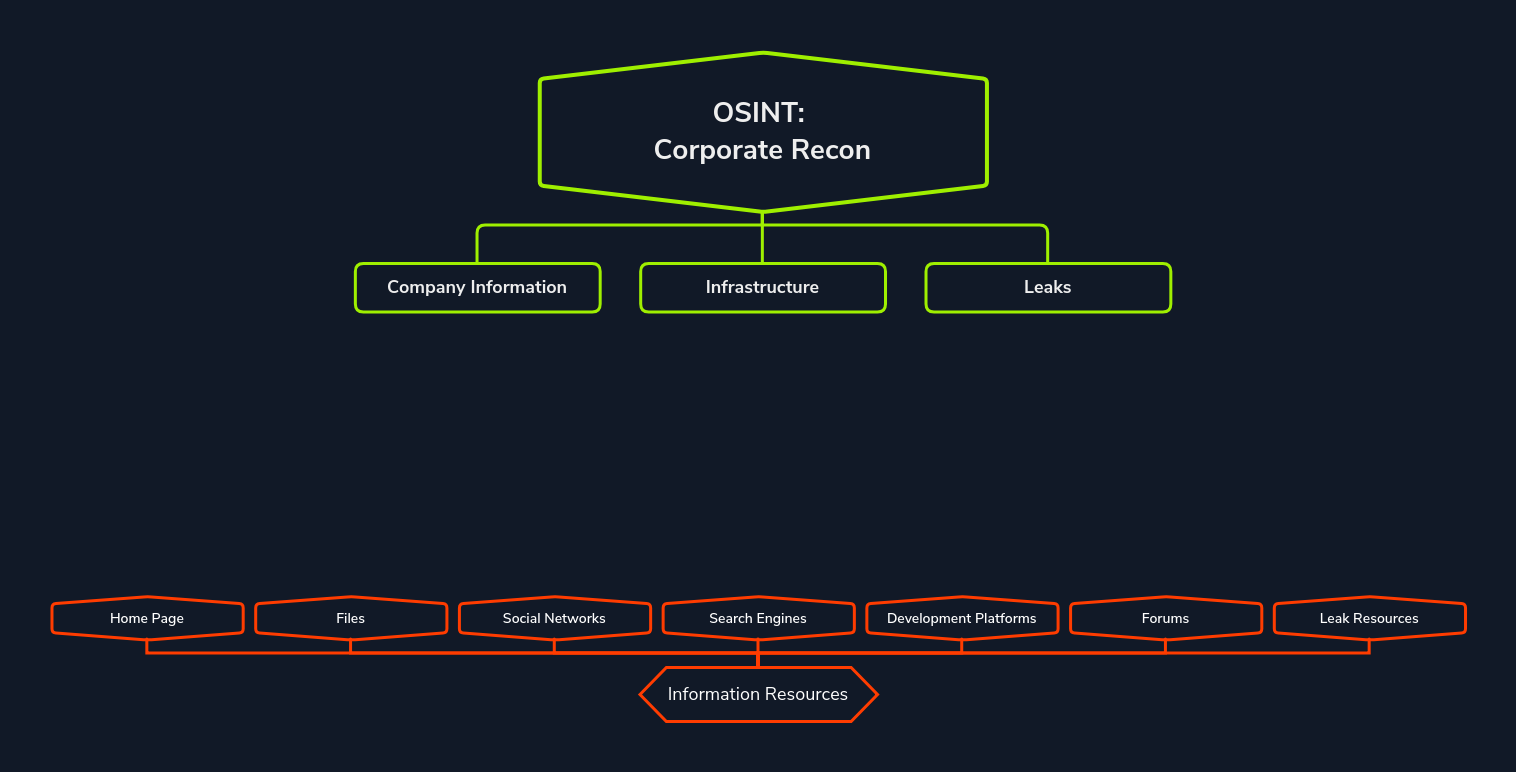
\includegraphics[width=\linewidth]{recon/osint/images/osint-structure.png}
  \caption{OSINT structure}
  \label{fig:osint-structure}
\end{figure}

Here we distinguish between the {\bf Core Elements} we need and the {\bf Information
Resources} from which we can extract the corresponding core information.

{\bf Core Elements} are pieces of information that give us a better picture of
the company and its infrastructure. These can be names and versions of software
applications, servers, names, user names, hashes, URLs, passwords, and much
more.

{\bf Information Resources} are resources from which we obtain these Core
Elements. These information resources can be websites, social networks,
documents, scripts, and many others.


we have to keep in mind that any information we find will lead to repeated
searches and new resources for more detailed information. 

Therefore, it is highly recommended to organize the whole process in {\bf
cycles} and repeat the search with the new information for each new cycle. This
systematic approach allows us to have a structured workflow and clean
documentation that will enable the client and us to understand precisely how
the data and information have been obtained.

When we use OSINT, we can divide our core information results into three categories:
\begin{verbatim}
Company Information 	Infrastructure 	                Leaks
Organization 	i       Domain Information 	            Archives
Locations 	            Public Domain Records 	        Internal Leaks
Staff 	                Domain Structure 	            Breaches
Contact Information 	Cloud Storage
Business Records 	    Email Addresses
Services 	            Third-Parties
Social Networks 	    Compounded Social Networks
                    	Technologies in Use
\end{verbatim}

In this methodology, we take a point from the information categories ({\bf Core
Elements}) and search for the relevant information for it through the different
{\bf information resources}.

Theoretically, the reverse procedure can be used too. However, it has a
significant disadvantage because we have many information resources to adapt
our methodology to, rather than our information resources to our methodology. 

The result is that we are left with an unstructured approach and are guided by
the information resources but not by the information results.

\subsubsection{Workflow}

{\emph It is essential to understand that, using this methodology, we adapt our
information resources to the methodology, not the methodology to our
information resources.}

In this way, we work according to an organized structure and get far more
results. It requires a little more effort to go through the same page several
times to cover different information areas and categories (Core Elements).
However, we maintain a structured and transparent methodology without
overlooking specific details relevant to a particular information area and
category. This also allows us to create clear and detailed documentation and
work in cycles independent of the cases.

To make this structured methodology efficient, we need to work with two browser
windows: 
\begin{itemize}
    \item {\bf Research Browser} use only for our research. Here we send all search
        requests and log the entire OSINT process. The research browser's
        history must be cleaned before use to prevent us from logging results
        from other companies. We can use the add-on called
        \href{https://github.com/jiacai2050/history-master}{History Master} to
        log our searches and finally export them as documentation.
    \item {\bf Resource Browser} serves as a summary of the information
        resources we find during the investigation. In this one, we move all
        the information resources to which we can return to search for
        information for other categories. For example, we will get to know
        development platforms containing leaks and names of employees or
        developers, email addresses, and usernames. In this part, we can also
        use the add-on called
        \href{https://addons.mozilla.org/en-US/firefox/addon/single-file/?utm_source=addons.mozilla.org&utm_medium=referral&utm_content=search}{SingleFile}.
        This allows us to copy the web pages with the information and save them
        locally as proof.
\end{itemize}

he actual process is quite simple, as we now split our results between two
browsers. So as soon as we have found a new information resource and examined
it in the Research Browser and discover that there is more useful information
there, we drag the newly opened tab to the Resource Browser, which we will turn
to later.


{\bf We document all our discoveries and structure them accordingly to each
phase and our cycle.}


\subsubsection{Logging}

To work efficiently and in a structured way, we must also document the results
and information we find clearly. However, we also need to log our steps and
prove how we found the information. With the two different browsers, we have
found a way to separate our search from the resources. To create clear
documentation, we need three components:
\begin{itemize}
        \item Visited websites
        \item Timestamp
        \item Queries
\end{itemize}

All of this information is stored in our browser history, and we can use it
quite efficiently for our purposes. A handy add-on for this is History Master.


Usefull tips :
\begin{itemize}
    \item export history-master to csv then \verb+csvtojson < history.csv | jq .+
    \item We can store all the websites locally using the SingleFile. This
        add-on offers an excellent way to download all open tabs with one
        click. Another great advantage of this is that these stored pages can
        also be searched locally \verb+cat *.html | html2text | grep "Emma Williams"+
\end{itemize}

\subsection{Business Investigation}
We should note down or at least keep in mind some questions that will help us
get a clear and efficient overview during our research. These questions will
also help us establish links between the individual pieces of information that
the actual intelligence piece of the phrase OSINT stands for.

\subsubsection{Company Information}
includes the company's general overview. This means
we will try to understand the company's structure:
\begin{itemize}
    \item  How many employees does the company have?
    \item  What is its objective?
    \item  How is the company positioned in society and the market?
    \item  How profitable is the company?
    \item  How does the company function?
    \item  How do they manage their tasks?
    \item  What services does the company provide?
    \item  How is the company positioned financially?
    \item  Which target group does the company pursue?
    \item  Where is the company located?
    \item  What are the physical security measures?
    \item  How do interaction and advertising with (potential) customers take place?
    \item  How strong is the company's reputation?
\end{itemize}

The process of staff investigation, can provide us with valuable information
that allows us to assess their knowledge and experience. It is a very
time-consuming stage to search for these people, as we first have to find all
the people then try to find everything relevant about them if allowed

In this search, we try to determine:
\begin{itemize}
    \item  What position do the employees hold?
    \item  Which departments exist within the company?
    \item  Their day-to-day tasks.
    \item  What are they responsible for?
    \item  What dependencies do the employee have?
\end{itemize}

Here we will only deal roughly with the individual employees. We will deal with
them more directly in another Module called {\bf OSINT: Staff Investigationr}.
It requires a slightly different approach to work with the information in an
efficient and structured way. Once we have gathered this information, we will
move on to profiling, which we will deal with more extensively in the {\bf OSINT:
Staff Profiling Module}.

Social networks are used for personal profiles and the sharing of information
from one's own private life. They are also used to publish products and news
that provide new information about the company and its technologies. Therefore,
in this phase, we try to determine:
\begin{itemize}
    \item Which products are being developed?
    \item Which technologies are utilized?
    \item Who are the developers?
    \item Which conferences do the employees attend?
    \item Where are these products used?
    \item Who uses these products and services?
\end{itemize}

For example, when new software is released and sold to thousands of companies,
it is interesting to get a demo of that software and analyze it for
vulnerabilities. If we can identify a vulnerability, all companies that use
this specific software version will also be affected by the vulnerability.

\subsubsection{Infrastructure}
we move into more technical details. Here we try to find
out:
\begin{itemize}
    \item  How is the company set up in terms of information technology?
    \item  Who are the administrators?
    \item  Does it meet the best possible security standards?
    \item  Which technologies are used?
    \item  What entries are there about the domain?
    \item  Which certificates can be obtained?
    \item  How many domains are registered to the company?
    \item  What is the ASN?
    \item  Which netblocks has the company reserved?
    \item  Which third-party providers are used, and for what?
    \item  How many and which servers are publicly accessible?
    \item  How many and which email addresses are available?
\end{itemize}

This gives us a much better understanding of the technologies and the technical
environment we have to deal with. Understanding how the entire company is
positioned from an infrastructure standpoint is essential for identifying
potential attack vectors. For example, specific configurations in the DNS
servers can give us a rough idea of how experienced our target company's
respective administrator is.


\subsubsection{Leaks}

Most of the data put on the internet is stored there for decades and can be
found easily. We can find different versions of the web servers and the
website's design, for example, or documents removed years ago that contained
up-to-date information about employees, technologies, or processes.

Internal leaks can be found on various forums. When a developer on
StackOverflow asks a question to solve a problem in their code, the code is
often shared with the others to give better insight into their issue. If the
developer is under a lot of pressure or distracted, they may accidentally post
code containing passwords or other sensitive data. The functions that the
developers are working on can be much more interesting. These may contain
vulnerabilities if inexperienced developers are employed to write specific
sections of code.

\section{Company information}

\subsection{Organization}
When we talk about company information, we focus our interest on the points
that can give us a detailed view of the entire business and its processes. This
type of essential information is usually found on the target company's
websites. We will not necessarily find all the necessary information to give us
an {\bf insight} into the company and its {\bf processes}. This could tell us which
companies will be most interested in working with our target company and which
requirements must be met. Understanding our target company's business processes
can give us an idea of how to structure our attacks. Therefore we can design
our attacks to be executed during a specific step in the process.

We can also get an insight into the company's dependencies. From this, we will
be able to conclude which technologies are needed to manage the company, which
will indicate how the company may be structured from an infrastructure
perspective.
\begin{figure}
  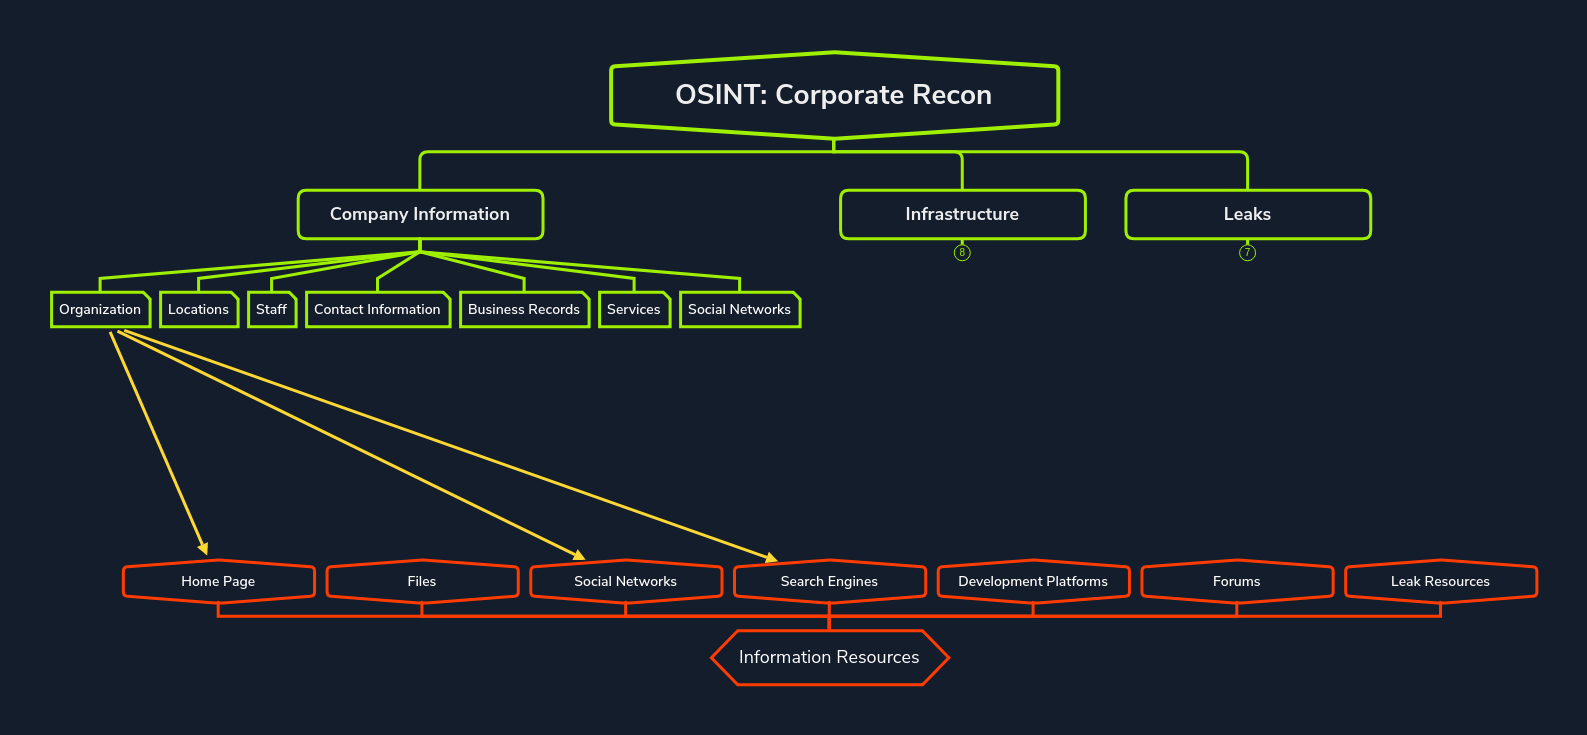
\includegraphics[width=\linewidth]{recon/osint/images/osint-org.png}
  \caption{OSINT Organization}
  \label{fig:osint-org}
\end{figure}

Generally, the company's home page, social networks, and search engines can be
used to map out the company's organizational structure. There are no useful
tools that can be used to map out the company's organizational structure
efficiently. Instead, we must rely on the logical association between the
information we will find during OSINT and the actual intelligence.

Furthermore, it is challenging to keep it dynamic because every company has
unique staffing needs and employees, all of whom bring different strengths,
weaknesses, and abilities. Therefore this field of OSINT is more a repeatable
process than a static method.

\subsection{Locations}
If our engagement is a red team assessment, then such information is much more
relevant than a regular penetration test procedure. Red-teaming can also
include, among other things, the physical security of the company and is used
to determine which methods and techniques can be used to obtain highly
sensitive information that may not be accessible from the internet. The
company's locations are of great importance for this. However, the scope and
rules for which procedures may and may not be used must be strictly observed.

Companies already pay a lot of money to attract potential customers by
presenting themselves to their customers in the best possible way and sell
themselves better from a marketing point of view. Here we can always ask
ourselves when the company would arouse our {\bf interest}.

\begin{figure}
  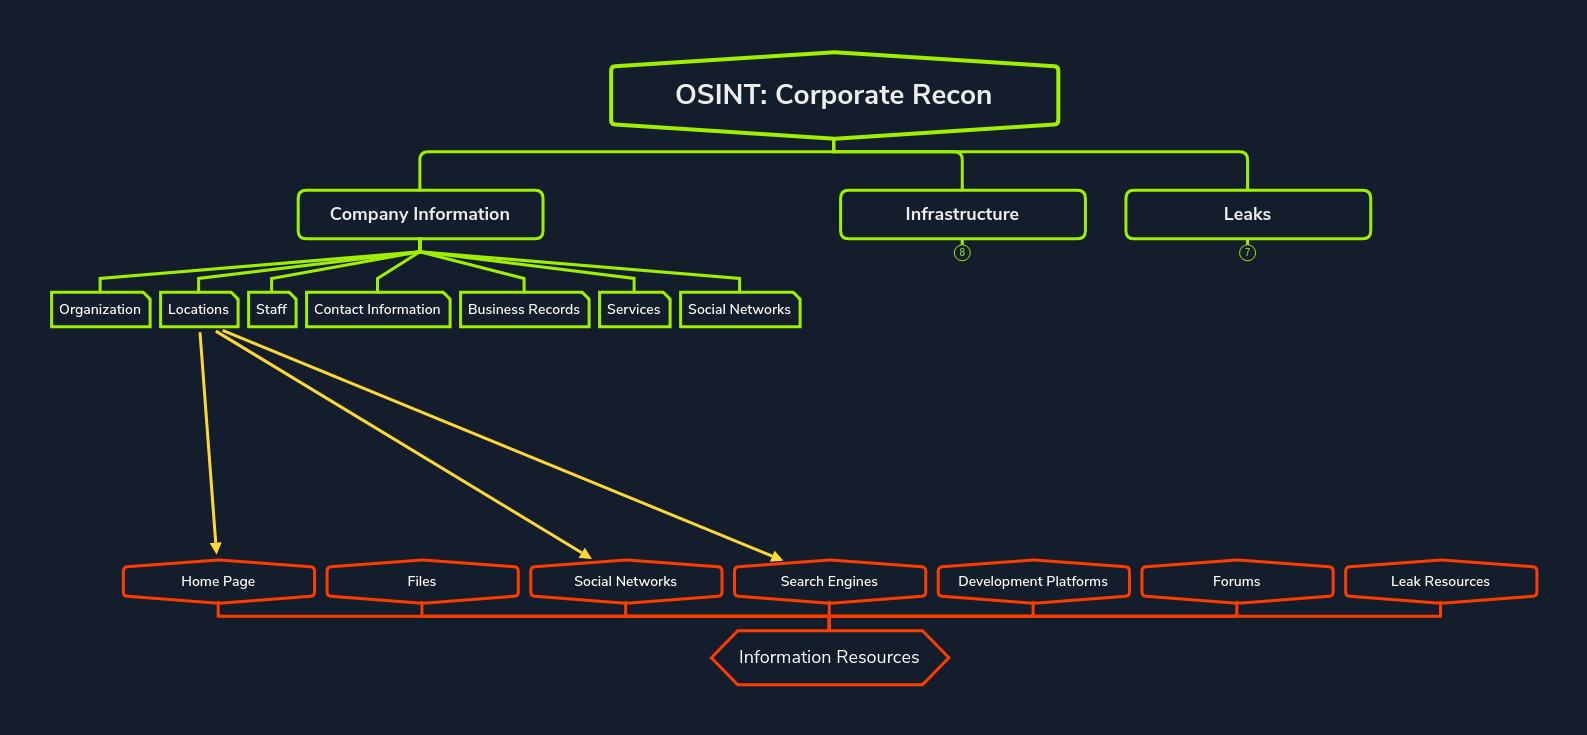
\includegraphics[width=\linewidth]{recon/osint/images/osint-locations.png}
  \caption{OSINT Locations}
  \label{fig:osint-locations}
\end{figure}

When we look into a company's locations, we have to identify the most obvious
locations in advance. Larger companies that are active in the field of
production sometimes have sites that they do not mention. These can also be
identified in the OSINT process. The most prominent locations are usually
listed on the company's home page. After all, the company wants to attract
potential customers with the number of locations it has. It is an overall
strategy for companies to present themselves as the best all over the world.
This contributes significantly to marketing and increases the number of
customers and thus the turnover.

In general, we can find basic information about a company's locations in
advance using the following resources

\subsubsection{Home Page}
If we start with the home page and browse through the site a little, we will
find {\bf countries}, {\bf cities}, {\bf addresses}, and possibly even maps
that show the company's locations. 

Most of the time, we will also find lists that include the countries and/or
cities where the company has its offices. These locations are usually managed
locally by administrators but also may be managed centrally. If the company is
centrally managed, these locations (either the entire company or specific
locations) within the scope can also provide us with attack vectors that we can
use to get into the systems' central administration infrastructure.

\subsubsection{Social Networks}

Social networks are used to share much information, especially information that
potential customers can use to learn more about the company. This includes the
publication of locations of offices or production facilities. This type of
information can be found on many social networks such as Twitter, LinkedIn,
Instagram, Snapchat, YouTube, WeChat, Facebook, and others. Most links to a
company's social networks can be found on their home page.

\subsubsection{Search Engines}

Every company location can provide us with another potential attack vector,
whether physical or technical. Each site has different employees and managers
who have their way of working and can open up different attack paths for us
than other locations. As soon as we have detailed information about the
locations, we should document them and, in the best case, add a graphical
representation as evidence in our documentation. For example, we can use
\href{https://maps.google.com/}{Google Maps},
\href{https://earth.google.com/web/}{Google Earth},
\href{https://showmystreet.com/}{ShowMyStreet}, and many others to obtain these
types of views.

In this case, we could pretend to be a significant client for potential
collaboration and organize a meeting to be let into the building and get a much
better insight into the company's processes. If the contract requires a
physical test, we can also get an inside view of the building's physical
security, such as door locks, windows, security, cameras, rooms, departments,
and more.

Information about locations is mainly interesting for {\bf physical Red Team}
operations. This is because it distinguishes between the times at which a
"break-in" can be most efficient. If a physical assessment is conducted during
working hours, we must be granted appropriate access to restricted areas
upfront. If possible, it is better to find a way to enter the building at night
if the alarm systems and their vulnerabilities allow it. The locations
themselves are the company's buildings and the location of the offices.
Sometimes there are also badge readers that we can see and use to identify how
to set up our cloner to hijack access cards wirelessly.

Suppose a manager or even higher employee feels safe in their office, which has
only access to a minimal number of employees and suddenly finds a USB stick on
their desk. In that case, they may wonder where it came from. The feeling of
being safe increases the likelihood that the USB stick we leave behind will be
plugged into their computer.

In larger companies, we will find some of these locations, which at first
glance already indicate some potential weaknesses in the field of physical
security. Suppose we have such an assignment where we also have to test the
organization's physical security. In that case, we can use the same resources
to get a picture of the terrain or even physically walk through the location as
a "passerby" and record a video of the terrain with a simulated phone call.
Depending on whether the location and the terrain allow it, we can also take
photos from a distance. By using the online resources, we will also be able to
gain some information.

We have to keep in mind that these photos have not been made today and may not
be up to date. Nevertheless, if we take a closer look at them, we can see some
interesting characteristics of the building, which could be helpful for us.


\subsection{Staff}
Every company's marketing department attaches great importance to the best
possible representation of its {\bf staff} so that potential customers can be
sure they will be taken care of in a professional manner. The company's
employees handle all the processes. We are interested in the information they
use to interact with the company and its infrastructure. This may include but
is not limited to email addresses, phone numbers, usernames, passwords, and the
social networks on which they operate.

The employee's role in the company can also be used to assess their privileges
in specific areas. Thus, a manager would likely have higher rights than
customer support. However, even if a secretary does not have direct access to
the systems, the individuals in these roles can be an attractive attack vector
for us since they most likely have full access to calendars, plans, contact
data, email addresses, and more.

\begin{figure}
  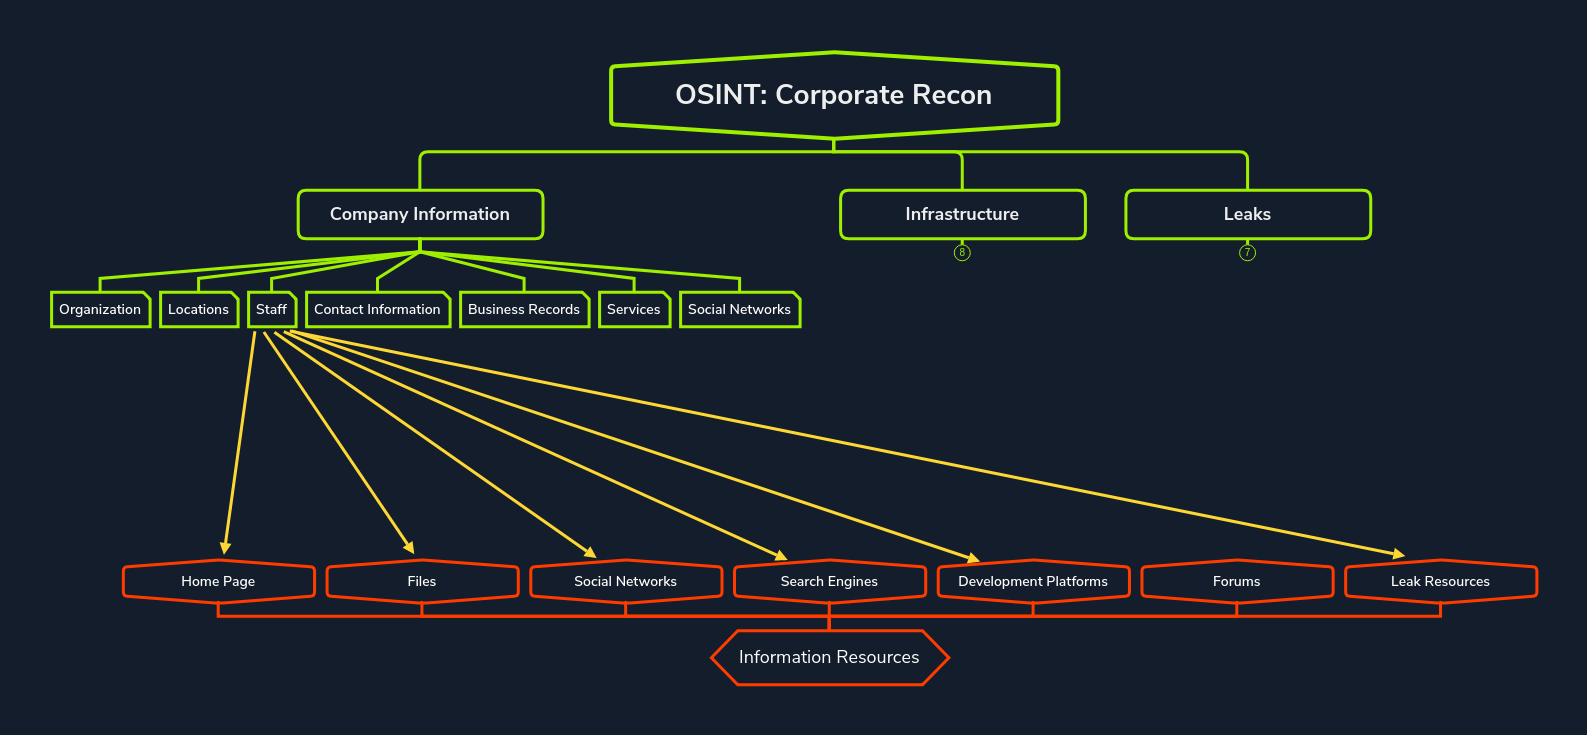
\includegraphics[width=\linewidth]{recon/osint/images/osint-staff.png}
  \caption{OSINT Staff}
  \label{fig:osint-staff}
\end{figure}

Information about the company's employees and managers is essential for us,
enabling us to reconstruct the internal corporate structure. With this
information, we will be able to identify the different departments' managers
and design our social engineering attacks better and more efficiently. We are
not yet looking at individual employees, but rather looking at who is employed,
who is in charge of what, who is responsible for what, and try to get a picture
of the internal communication flow.

The methodology we have used so far can also be applied to staff. However, this
field covers many potential attack vectors for {\bf phishing campaigns} and
{\bf social engineering} attacks, which we need to filter out. We will get many
valuable results, but this does not cover everything applied to the staff. This
field will be discussed in more detail in the Module {\bf OSINT: Staff
Investigation}.

In this step, we should continue to focus on getting an overview of the
company's employees to gain insight into its internal structure and hierarchy
and to be able to reconstruct it if necessary.

There are many sources we can use to obtain this information. Among them are
the following

\subsubsection{Home Page}
Most of the time, we can find the company's essential contact persons on the
"About Us" page. These staff members are usually trained to present themselves
professionally to customers and have the necessary answers to the most critical
questions.

It is interesting to note that we can read a biography for the C-level staff
here. This can serve us very well later in social engineering to find common
topics we can discuss and gain a certain amount of trust and sympathy from the
relevant persons. An important thing to note here is that these people would
only deal with large customers who promise a significant profit. Otherwise, it
can be hard to get directly to them.

We are interested in the employees who are already employed and want to know
what types of employees the company is actively recruiting. IT offers many
different specializations, enabling us to identify which technologies the
company works with or plans to work with by reading through open job
requisitions. Therefore we can continue to search for job offers on the
homepage that are still open or on the company's LinkedIn profile.

\subsubsection{Files}
Often companies offer different flyers, reports, and news in the form of files.
The software used to create these files is usually registered and only
available to authorized employees registered in the system. This data also
includes the software that labels the created files with metadata. These can
then be extracted and read out with the help of exiftool~\ref{tool:exiftool} or
metagoofil. This
information can include usernames, dates, software and version numbers,
geographical coordinates, and much more. We should download as many accessible
files as possible and extract the metadata accordingly.

\subsubsection{Social networks}
Finally, most employees do not want to miss the opportunity to get better job
offers from other companies and keep their profiles updated on business
networks. Maybe even with the latest projects they had to deal with to show off
their skills. Every company wants to have the best possible presence on social
media and, therefore, publishes links to their company profiles. These are
often also linked to the profiles of all their employees. One such source could
be LinkedIn, for example.

Apart from the individual employees and their profiles, LinkedIn can also give
us a better overview of our target company. For example, we can find out an
estimated number of employees for our target company.

On LinkedIn, we can also enter specific keywords in the search field, which
will filter the target company employees to make our search more specific. We
need people who work on computers and typically are not interested in those
that do not use a computer at all in their day-to-day jobs.

inally, we have filtered out our potential targets very well and have specific
ones to focus our attention. All business and social networks will be covered
in a later section. Other valuable sources for employees and job positions
are:
\begin{verbatim}
Xing 	
Monster 	
Indeed 	
Glassdoor 	
TrustPilot
\end{verbatim}

iFurthermore, we can use {\bf search engines} we know from which we will
discover other employees, the social networks on which they appear, the {\bf
development platforms} used by developers, and other files from which we can
extract metadata. We can obtain further information through these {\bf internal
leaks}. The search for employees requires an adapted approach and represents an
additional larger field of information sources. It is crucial to examine them
separately. Otherwise, we might get stuck in this phase. This will become much
clearer in the {\bf OSINT: Staff Investigation Module}.


\subsection{Contact Information}
Another critical point for all potential customers is the company's
accessibility. For this reason, {\bf contact details} are always disclosed.
After all, customers may want to find out more about the company or even
arrange a meeting. Contact information includes phone numbers and email
addresses, and usernames from various communication portals such as Skype,
Microsoft Teams, Slack, Discord, etc. These usernames can also be associated
with the employees. This part of OSINT will be discussed in more detail at {\bf
OSINT: Staff Investigation}.

\begin{figure}
  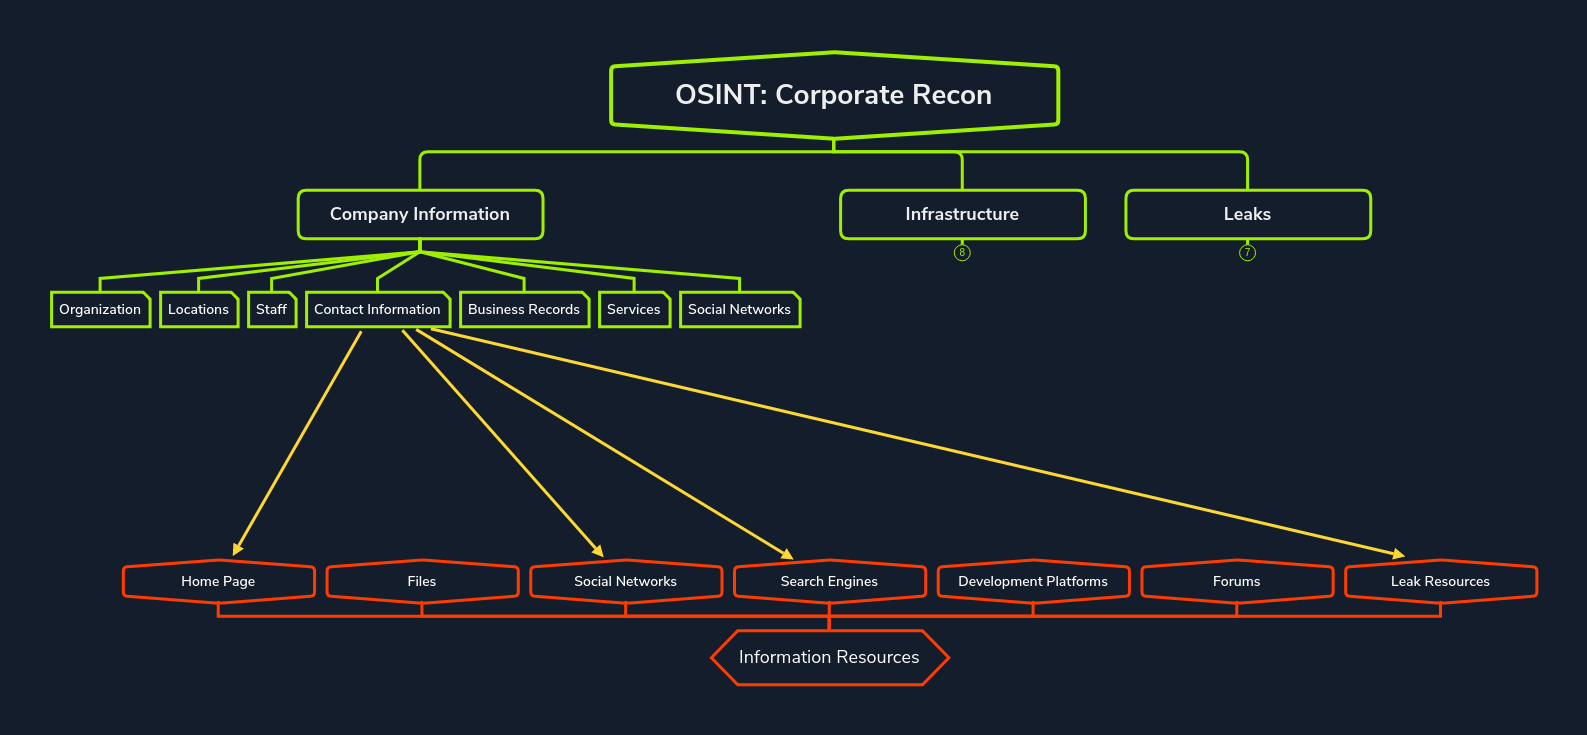
\includegraphics[width=\linewidth]{recon/osint/images/osint-contact.png}
  \caption{OSINT Contact}
  \label{fig:osint-contact}
\end{figure}
Contact details may be relevant to contact the appropriate person and send
inquiries to find out more about the company's processes. These may include
technical issues where we want to ensure that the products we offer will work
with our working environment.

\subsubsection{Home Page}
For example, in the next Penetration Testing phase, we could call the {\bf
phone numbers} to pretend to be customers of the company, ask short technical
questions, and ask them to help us with our issues. It is also interesting to
note that larger companies often have more than one domain. Therefore, the
contact persons' {\bf email addresses} may be on a different domain than the
one on which the main website is located. We could, for example, use these to
prepare our phishing campaigns and use these email addresses as targets.
Phishing attacks can provide us with sensitive information, such as passwords
or usernames, which can be very helpful, if not essential, in our penetration
testing process.

This information is crucial for us, especially for phishing, vishing, and
social engineering attacks in the {\bf Exploitation phase}. Employees from the
customer service and sales teams communicate a lot with (potential) customers
and therefore easily fall into a routine requiring repetitive processes. By
human nature, routine operations reduce the attention span, leading to the
inattentive and careless performance of their tasks. This is one of the
weaknesses that we can use for our purposes when we talk to an employee and
influence them to click on a link we send him.

\subsubsection{Social Networks}

Social networks provide us with a platform for interacting with the company's
employees and offer a wide variety of information about them. It is irrelevant
whether these are private social networks or business networks. What is
important is that we can obtain additional information through each of these
networks, including {\bf contacts}, {\bf partners}, {\bf co-developers}, their
{\bf phone numbers}, and {\bf email addresses}.

\subsubsection{Search Engines}

It is also beneficial to note down all the persons' {\bf names} because they have to log in to their domain with the respective identifiers or unique name format. IT people are especially interesting because most companies allow IT people to do their work from home. This indicates that there must be a specific type of remote access mechanism for connecting to the internal network remotely.

Another excellent source to find out the email addresses of the target domain
is \href{https://www.hunter.io/}{Hunter.io}.

We can verify each email address via \href{https://emailrep.io/}{Emailrep.io} and check how the mail servers handle it.
\begin{verbatim}
curl emailrep.io/<firstname>.<lastname>@<domain>.<tld>
\end{verbatim}

\href{https://rocketreach.co/}{RocketReach} allows us to identify email address formats by domain and the other email addresses linked to the corresponding managers. It is a paid service provider, but the results we get from it are very accurate, and it is an excellent way to find out links to the company's employees and the platforms they use.


\subsubsection{Leak Resources}

When we talk about leaks, we are not just talking about published databases
that contain users' passwords and email addresses. Apart from the fact that
these databases offer an excellent research opportunity, if we know the domain
to which the email addresses are registered, we can also find new and unknown
email addresses.

Apart from that, \href{https://web.archive.org/}{WayBackMachine from
Archive.org} offers us a very effective way to search for contact information.
It shows us older versions of the company website when IT security was less in
focus than today. Before a company becomes large, the bosses establish
themselves much more in all the necessary processes to efficiently control
them. Therefore, email addresses were often published on the websites at that
time to establish contact with the managers and customers better. However, in
most cases, these email addresses are rarely changed by bosses and
highly-positioned members. Therefore, we need to review snapshots of the target
company website on WayBackMachine as part of the OSINT process. Below is an
example of the various snapshots taken for a sample target company. Browsing to
one of these would show us the state of the company website on the given date,
which may differ significantly from the current website version and provide us
with useful information or even expose hidden functionality.

\subsection{Business records}
Significant customers look at the company's website and the {\bf business
records}, to learn more about it. From an OSINT perspective, they can also tell
us a lot about its progress. These include the company's {\bf locations}, {\bf
financial situation}, {\bf references}, and {\bf reputation}. We are
particularly interested in poor feedback about the company.

Poor feedback requires poor communication and the resulting i{\bf failures in
the business processes}. If a customer's inquiry or request is not fulfilled,
it may not always be a human mistake on the part of the employee but may
indicate technical issues. Companies often try to "hide" this feedback not to
create a wrong impression for potential customers.

Business records also include the degree of recognition in the market. For
example, we can get this through reviews by (former) employees or on social
networks. Customer satisfaction also plays a role. We can conclude how
structured and coordinated the company works internally to complete its
services and overcome customer problems for the services provided.

The company's financial situation tells us a lot about its commitment and
productivity. If a company continually offers new products and services, it can
positively affect its financial situation. Depending on the company's size, the
downside of this is that it can lead to chaotic processes. This can mean a
great deal of organizational effort and communication. Therefore, it leads to a
higher risk of phishing attacks because the content of a detailed, customized
phishing email is rarely actually checked.

\begin{figure}
  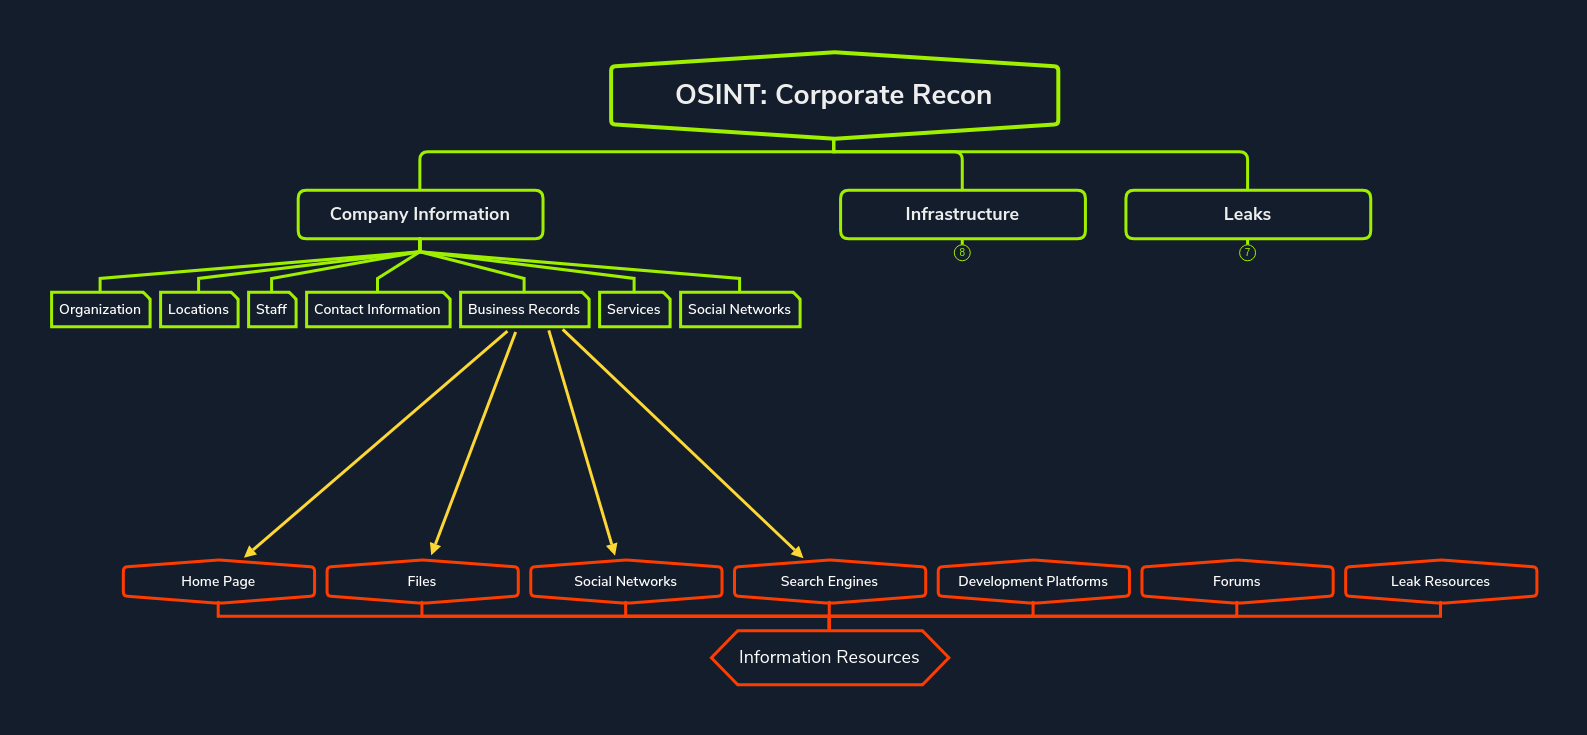
\includegraphics[width=\linewidth]{recon/osint/images/osint-business-records.png}
  \caption{OSINT Business records}
  \label{fig:osint-business-records}
\end{figure}

\subsubsection{Home Page}

{\bf Financial records} can give us a good overview of how the company is doing
and how it is currently growing. It also gives us information about what the
company depends on and whether it is presently healthy from a financial
standpoint. As soon as a company is under high pressure, it naturally tries to
save as much money as possible. These types of financial constraints often
force companies to seek out lower-quality services from third parties. It does
not matter whether these services are technical or not. With lower quality
services, it is more likely that they do not meet the highest security
standards and that we will be able to find some information about our target
company.

\subsubsection{Files}

Files that we can find on the internet contain not only potentially important
metadata but also general information. Every company must present itself
efficiently and profitably. After all, they want to attract new customers and
show their success to convince them to give them their business. Many companies
demonstrate their success through financial reports. These can be found on the
company's website or are sent to subscribers via newsletters.


Using Google search, we can find and filter out files like .docx, PDFs, and
others. We can use Google Dorks for these purposes. A small list of the most
important "dorks" can be found
\href{https://securitytrails.com/blog/google-hacking-techniques}{here}.

\subsubsection{Social Networks}

In addition to finances, the company's culture also plays an essential role.
This enables us to determine how certain situations are handled and how
reliably the processes function. Suppose a 3rd-level support staff member is
neglected and frustrated with their company's management concerning their
position. In that case, it is a very strong demotivator that consequently
reflects on their performance, attention, and attentiveness. This employee will
most likely put in far less effort and even less thought into the company's
future.

With the help of Google, we can find more reviews and reports about the
company. This will help us identify where the most difficulties and problems
occur in their processes that we can focus on later. It is essential to note
the perspective from which the reviews have been written. They can be written
either by customer or an employee. When we Google the reviews, we will find
sources such as Indeed.com, which gives us an excellent opportunity to look at
the reviews to get a better idea of the atmosphere and process.


\subsubsection{Search Engines}

On \href{https://www.crunchbase.com/}{Crunchbase.com}, we can find some of the
published records concerning our target company. Often we can find financial
reports from which we can find more helpful information. These reports also
list some information about employees.


If our customer is a publicly-traded corporation, it is even easier for us to
track its financial status. This is because we can view detailed information on
them on \href{https://finance.yahoo.com/}{Yahoo! Finance}.


For us as penetration testers, it is enormously important to look behind the
scenes and think outside the box. We need to understand how the company's
financial situation has developed and which data and factors have contributed
to this. If we know these, we can start to trace their management processes and
go into more detail to understand what steps were necessary and how we as
"attackers" could influence them by penetrating the corporate network.

\subsection{Services}
{\bf Services} are also explained in great detail on the website so that the
number of external inquiries is kept to a minimum. For this reason, how each
service is carried out is usually discussed in detail. All other questions that
arise are generally specific.

\begin{figure}
  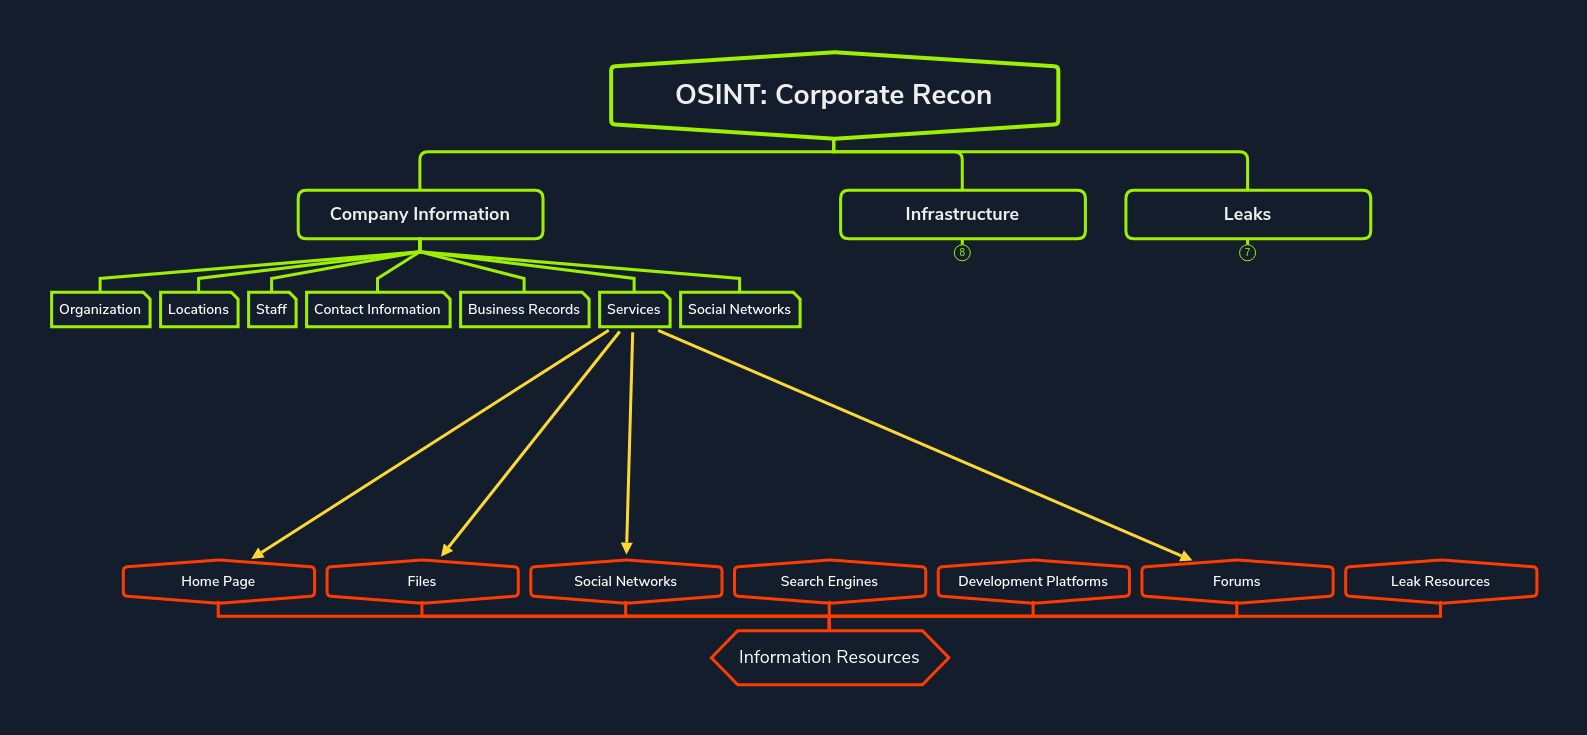
\includegraphics[width=\linewidth]{recon/osint/images/osint-services.png}
  \caption{OSINT Services}
  \label{fig:osint-services}
\end{figure}

\subsubsection{Home page}
On the product and service descriptions page, we will often find step-by-step
instructions that describe the entire process between the customer and the
completion of the service or the receipt of the product. Utilizing options that
are sometimes provided, such as the localization of the representative offices
and contact persons, we can also find, among other things, tools that the
website visitor can use.

These services may include information about the {\bf technologies}, their {\bf
workflow}, {\bf employees} who take care of these services, and resources that
may contain potentially security-sensitive information.

Suppose we are not familiar with the industry but want to find out how these
processes and orders are set up and managed. In that case, we should search
through the internet to find out what options are available and look at {\bf
similar providers} who may provide additional information. We must remember
that all companies in the same industry are usually competitors. At the same
time, the desire to be the \verb+#1+ in the marketplace brings the same desire to
provide the {\bf best possible services} to customers, which are often {\bf
very similar}. In many cases, the company also takes advantage of {\bf service
gaps} that the competitors do not or only poorly fulfill.

These are then often prioritized. This service is presented with much more information to show that this company is significantly better than the competition.

Nowadays, the management of services is done almost exclusively through a form
of software application. A high focus is placed on web applications and mobile
applications, making operation and control as easy as possible for customers.

\subsubsection{Files}

Information about the target company's {\bf partners} can also be found {\bf in
files}. This is because not all partners and technologies are presented and
disclosed directly. However, these companies may be marked as "{\bf Powered
by}" in these files.

As mentioned earlier, we can already see that our target company uses {\bf
cloud solutions} offered by the provider. This is also very valuable to us, as
we now know that we should be on the lookout for potential cloud-based storage
locations that may be publicly accessible.

\subsubsection{Social Networks}

In principle, social networks are used by companies for marketing purposes to
bring their products and services to the people and to draw attention to
themselves. Here, too, information about their services and solutions is
presented and published. In most cases, this is also linked so that these
solutions can be viewed directly and the company's website is visited. This can
play an essential role, especially with new releases of service solutions and
applications. If this has been tested poorly (or even not at all) for security
and vulnerabilities, then this application/solution represents a potential
attack vector.

\subsubsection{Forums}

A wide variety of technical discussions and news are discussed in forums. These
are very useful for us when we want to find out something about a company's
performance and services. Every post in the forum usually has a date when we
find out when an enhancement or application, or service was released. Based on
this time-lapse, we can roughly estimate how up-to-date specific software may
be. For example, if we find an application that uses a library containing a
vulnerability, we will be able to exploit it with the appropriate preparations
and measures. More information about vulnerable libraries and how many
applications are affected by those can be found in this
\href{https://www.veracode.com/blog/research/announcing-our-state-software-security-open-source-edition-report}{Veracode
report}.

Larger companies that have a large number of customers sometimes even provide
forums for customers. We can often register and peruse these forums. {\bf
Technical problems} are usually discussed there, and we can also ask questions
to find out more information. We can sometimes even see how the developers or
administrators solve specific problems. With a little bit of advanced
programming knowledge, we could even understand how a specific software-related
problem could be solved.




\subsection{Social Networks}
We can also ask where to find more information about the company during a phone
call. We are usually directed to {\bf blog posts}, {\bf videos}, or {\bf
documentation} from a marketing perspective that would give us better insight
into the company. We can find a variety of information about the target company
through the different social media networks. We usually first direct our focus
to the company's linked accounts via its home page. In turn, these may lead us
to different sources of information not mentioned on the home page.

We can also search the different platforms themselves to see where the company
is represented on social networks. Finally, we can use search engines or forums
to find out if the company is mentioned there.

\begin{figure}
  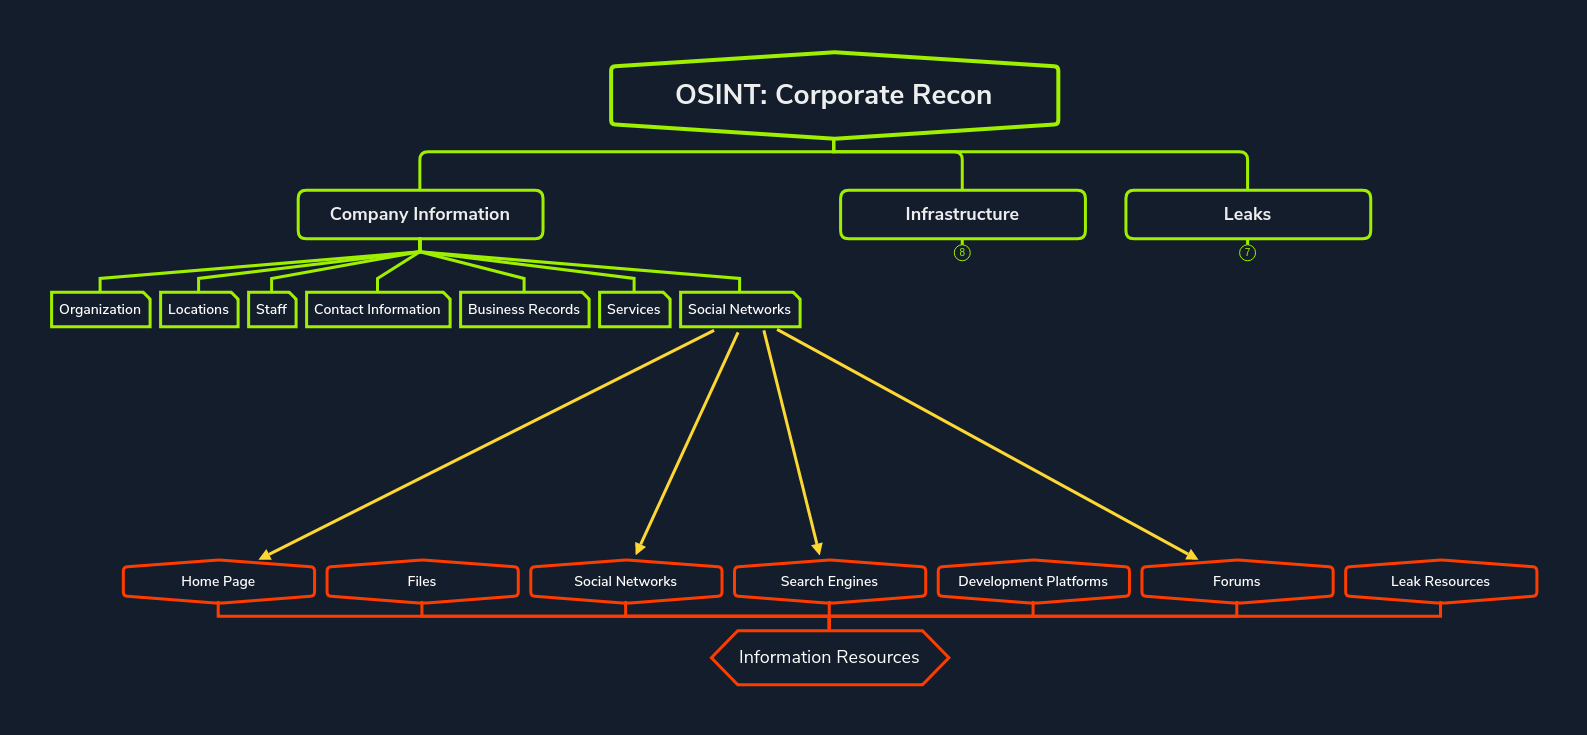
\includegraphics[width=\linewidth]{recon/osint/images/osint-social.png}
  \caption{OSINT Social}
  \label{fig:osint-social}
\end{figure}

With social networks, things can now get a bit more complicated and confusing,
as they serve as both information elements and sources of information. If we
look at social networks as sources of information, we enter what is known as
{\bf Social Media Intelligence (SOCMINT)}. To not lose the orientation and
overview of this, during the OSINT phase, we focus on the "movement" and
presence of the company's social networks. Therefore, in this case, we will
deal with the social networks and information elements. Once we get an overview
of the company's presence on the social networks, we can move into SOCMINT and
examine and analyze each platform in more detail.

To make the distinction clearer, we use social networks as Information Elements
(marked green) rather than Information Sources (marked red) in this phase. This
means that we are collecting the company's connections to social networks.

However, this does not mean that we have to limit ourselves here. We can combine both, but we have to keep in mind that we consider social networks as information elements (i.e., pure information for the company's value). We can find a lot of information about the company itself and its technologies. These include public and internal information but is not limited to:
\begin{verbatim}
Blogs/News 	Images & Videos 	Wikis 	Documents & Files 	Social Media
\end{verbatim}

\subsubsection{Home page}
Almost every medium-sized company strives to keep current and potential
customers up to date. In most cases, these sources are also straightforward to
find. After all, this news, which is also often published on blogs and social
media platforms, provides information about our target companies' progress and
success. This information is often provided to convince potential customers
that the company is always the best choice.

This news often includes new cooperations with partners and successes achieved
by the company. Additionally, new technologies and solutions for customers are
presented here that we should also consider. Soon we will look at a document
that may contain this type of information.

\subsubsection{Social Networks as Information Component}

Most companies see social media platforms as essential and indispensable from a
marketing point of view. In most cases, we find the links to the various
platforms directly on the website itself. On these social media platforms, such
as Twitter, LinkedIn, Xing, Facebook, Instagram, YouTube, and others, we find
not only the {\bf latest news} and {\bf developments} of the company but also
older posts that can give us information about the {\bf structure and
technologies}.

Another often overlooked component, which does not directly belong to the
social media category but fulfills the same purpose, is {\bf newsletters}.

\subsubsection{Search Engines}

All search engines also allow us to search for images and videos of the
company, which can also provide us with links to social networks and
information sources.

Companies often use {\bf images} and {\bf videos} to increase the
attractiveness of blog posts and news articles. In the last section, we have
already seen that we could identify a mobile application from a video and get a
short impression of how it looks. Now let's look at a picture of our target
company that provides us with some information.

i{\bf Photos} offer a far more significant security risk than most people
realize. Let us say we find a high-resolution photo of a company meeting where
the work {\bf IDs} are visible. Especially for {\bf red-team operations}, this
is incredibly beneficial because we can use the photo to recreate and prepare a
badge to get past the building's security personnel and get inside the
company's building.

The search for documents in this section is based on the fact that it allows us, among other things, to refer to sources on which social media platforms these files are stored.

A good start for finding documents and connections is Google. Using {\bf Google
Dorks}, we can define parameters that should be displayed. For this part, it is
enough to know that we can use the Google Dork "{\bf filetype:}" to define the
filetype that we are seeking. This results in output to links that explicitly
point to the specified file type of our target. Accordingly, we can download
and view them.

Do not forget that we must document each step and the corresponding source we
use to find the information. Otherwise, we will have difficulty describing how
and where we got this information from in the report.


Of course, we can and must also use other file types here. We will see later in
the section {\bf Internal Leaks} the valuable information these files can give
us, which can play a crucial role in the success of our engagement.

\subsubsection{Forums}
As mentioned earlier, forums serve as a good source of information for
technical difficulties and problems. Problems are also discussed and dealt with
on social networks. There are countless public forums such as Reddit,
StackOverflow, and others that the company can use for this purpose. Here, too,
we focus mainly on the presence of forums where people discuss our target
company.

Internal forums that we may stumble upon are very interesting to us. In these,
technical questions are answered in far greater detail than in public forums.
Therefore, we should keep an eye out if we can perhaps register on an internal
forum to search for information.

\subsubsection{Wikis}

The exciting thing about wikis is the information that is published and the
{\bf references} and {\bf external links}, which in turn point us to other
sources that can provide us with even more information. Some references and
resources can be Wikipedia, Github, or even {\bf internal/provided wikis} to
which it can be linked.

We can find a lot of helpful information from the wikis that describes the
company itself or its services. Wikis are created to provide detailed
information about specific topics and make them accessible to others. In other
words, they often serve as documentation that can provide valuable information
for us.

For example, we may find a post describing a specific application in detail
(i.e., how to install it, how to work with it, and more. We can determine which
    dependencies these applications have and can later use this information for
    Reverse Engineering to understand the developer better and uncover
    potential weaknesses.

\section{Infrastructure}
\subsection{Domain information}

Here we work our way piece by piece {\bf from rough to detailed} information.
Therefore we first have to get a technical overview of the company. Since we
usually already know the name of the company or even the domain name, this
information is generally sufficient to determine how the company is
structured.
\begin{figure}
  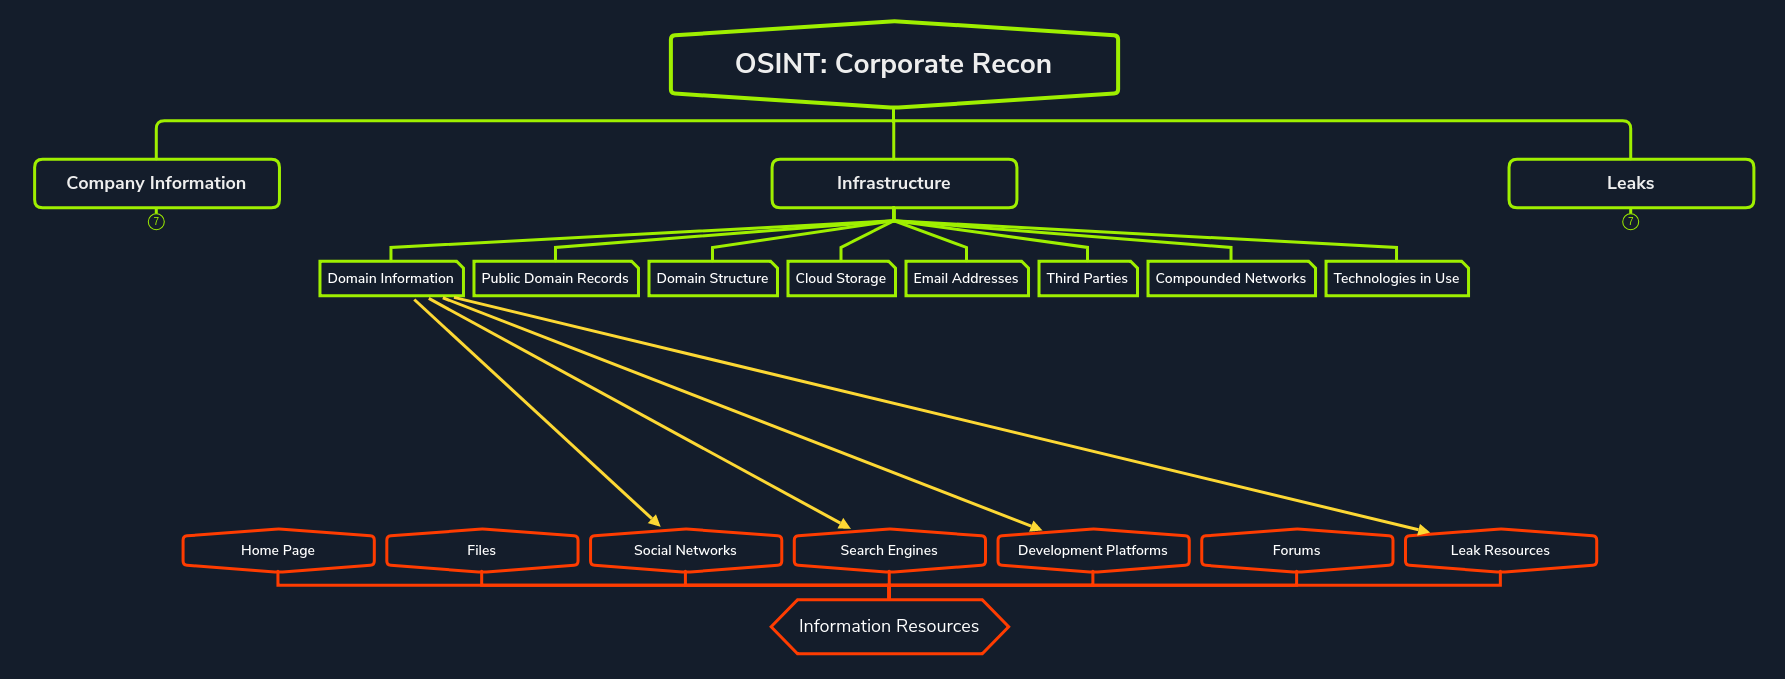
\includegraphics[width=\linewidth]{recon/osint/images/infra-domain-info.png}
  \caption{OSINT Domain information}
  \label{fig:osint-domain-info}
\end{figure}

The element we focus on in the first phase of the company's infrastructure
investigation is the domain names we can find. We then go into each domain and
get an overview of the subordinate structure that contains 
\begin{itemize}
        \item Netblocks
        \item Name Servers
        \item Mail Servers
        \item subdomains
        \item hosts/IP addresses.
\end{itemize}

We can classify the rough structure into three categories:
\begin{itemize}
        \item Public Records:  	
        \item Third Parties 	
        \item Domains
\end{itemize}

\subsubsection{Social Networks}
We often find references to domains or subdomains on social media platforms.


\subsubsection{Search Engines}
One of the most efficient methods of searching for domains is offered by
various search engines. In this case, we cannot focus on a domain name, but we
have to work with general company terms, such as the company name, the name of
the application or service, and others.

Another excellent way to find out information about our target domain is to use
a particular Search Engine Optimization (SEO) field called backlinks. 

One of such backlinks analyzers is
\href{https://app.neilpatel.com/en/seo_analyzer/backlinks}{Ubersuggest}.

\subsubsection{Development Platforms}
Development platforms also offer excellent information resources for us here,
as we will often find code that sometimes even provide information that is
dangerous for the company. This information can range from IP addresses and
hostnames, configuration files to credentials.

\subsubsection{Leak Resources}
Once we have a list of the company's domains, we can use it to look for known
anomalies that affect the company and the corresponding domain. One of the best
sources of information for this is
\href{https://www.virustotal.com/}{VirusTotal}, where we can scan each domain
for suspicious activity.


Another source that searches against many different developer platforms is
\href{https://searchcode.com/}{Searchcode}. It searches all possible codes for
terms that we specify in the search and shows us the sources accordingly.

\subsection{Public Domain Records}

Public domain records offer us excellent opportunities to trace the company's
information technology infrastructure structure. With the right arrangement and
knowledge of what the records are for and what information they contain, they
can provide us with information about the company's Internet presence. To get
this, we need to find out at least four components:
\begin{verbatim}
1. Netblocks / CIDR 	2. ASN 	3. DNS Servers 	4. Mail Servers
\end{verbatim}

This gives us an overview of which systems are accessible from the internet, in
which address range they are located, which IP neighbors they have, and how the
interaction between them takes place.

\begin{figure}
  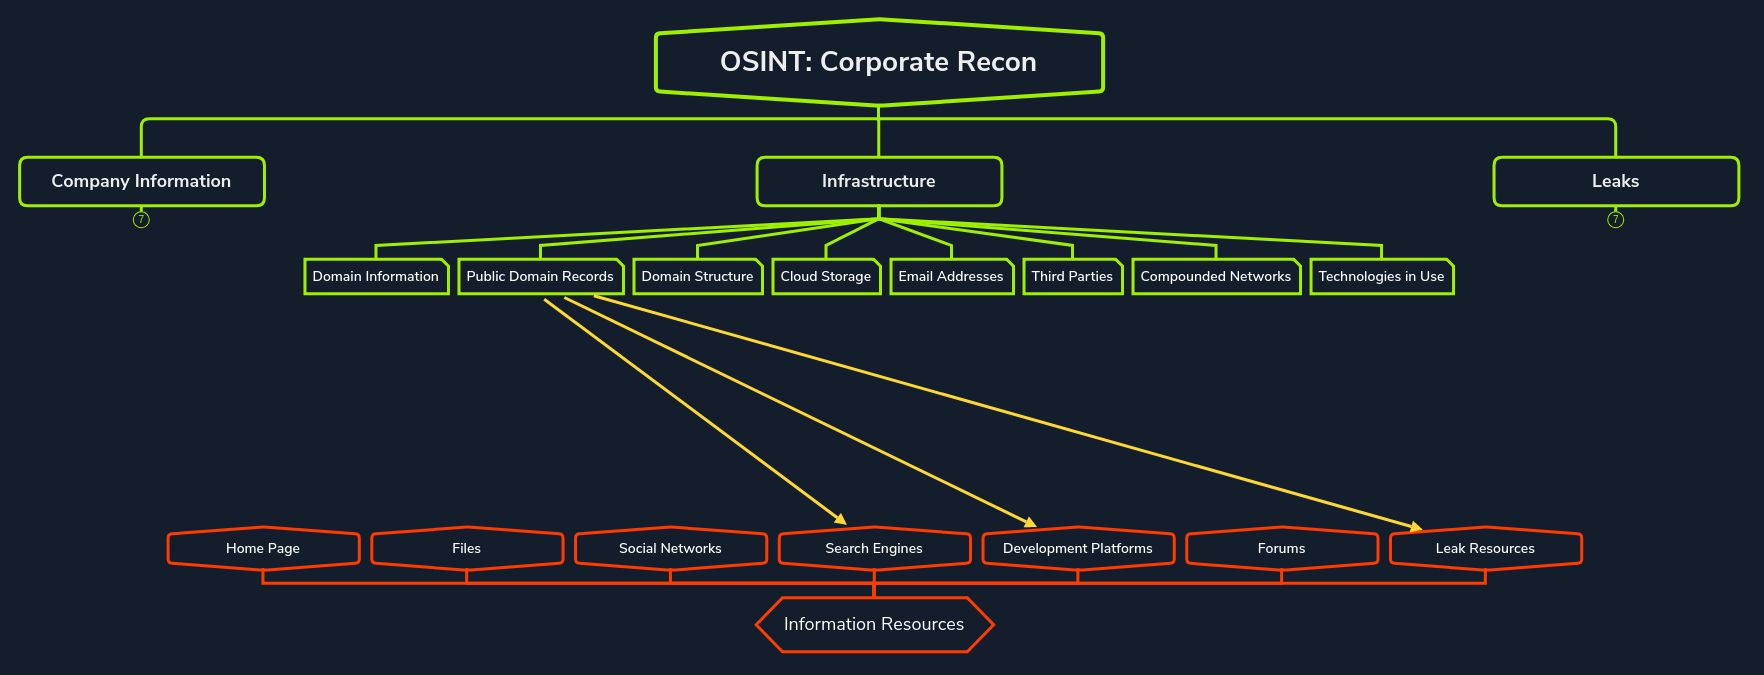
\includegraphics[width=\linewidth]{recon/osint/images/infra-pub-records.png}
  \caption{OSINT Domain public records}
  \label{fig:osint-infra-pub-records}
\end{figure}

\subsubsection{Search Engines}
The minimum information we need to get from our client, apart from the company's
name, is a domain or at least an IP address to start with. The scope of this
can vary greatly.

{\bf 1. Netblocks / CIDR}

During a black-box penetration test, our client will often only provide the
domain name. We can use this to find out a lot of helpful information. First of
all, we should find the IP address of the main webserver(s) and the IP address
range(s) / CIDR. For this, we can use the following command.
\begin{verbatim}
host www.inlanefreight.com
\end{verbatim}
Now that we have the IP address of the web server, we can find out which IP
address range it is located in. By default, we can work with the Whois protocol
used by a distributed database system to retrieve information about internet
domains and IP addresses and their owners.
\begin{verbatim}
whois 134.209.24.248
\end{verbatim}
We can also search the WHOIS databases for the company name. We are often given different identification numbers (mnt-ref), which we can use for further searches. These stand for the maintainer objects, which are used as a reference for the organization objects.
\begin{verbatim}
whois -B --sources RIPE,ARIN target-company
\end{verbatim}
We can also query the individual databases and identify the associated netblocks.
\begin{verbatim}
whois -h whois.arin.net target-company | grep -v "#" | sed -r '/^\s*$/d'
\end{verbatim}
Here is the \href{https://www.arin.net/resources/registry/whois/rws/cli/}{ARIN
list} of other flags we can use to get more information from
the maintainer objects. 


{\bf 2. ASN}

We can also see another crucial piece of information here, the {\bf OrigisAS}.
This is the {\bf Autonomous System Number (ASN)}. This number is unique and is
made publicly available so routing information can be exchanged with other
systems. This is done with specific IP prefixes, which we can use to find out
the netblocks ({\bf public ASNs}). There are also {\bf private ASNs} intended
for systems that only communicate via a provider. Other protocols such as the
{\bf Border Gateway Protocol (BGP)} are used if this is the case. We can use
\href{https://mxtoolbox.com/SuperTool.aspx}{MXToolbox} and its {\bf ASN Lookup}
option with the ASN to find out how many subnets the owner has.

Another way to get more information about the domain is to use the
\href{https://lookup.icann.org/lookup}{ICANN lookup}. Each domain is registered
to an organization or person with a unique ID, which provides information about
when the domain was created and expires.

{\bf 3. DNS Servers}

DNS servers are essential services today because they help the regular user
reach the web services they want.  It is often the case that companies own
several domains, and accordingly, these domains can offer different attack
vectors that can affect each other. The next step is to look at the DNS records
of our target domain using dig. Dig is a DNS lookup utility that can be used to
obtain publicly available information from DNS.

\begin{verbatim}
dig any inlanefreight.com
\end{verbatim}

If we now take a closer look at the records, we see that the SOA record shows
another domain, infreight.com. Therefore we will also look at these if the
scope allows us to do so. In this case, we assume that we have permission to
test this domain as well.

Another source we can use, which gives us a much better representation of the
DNS servers' records, is \url{https://dnsdumpster.com/}{DNSdumpster}.

Here we can see the entries for the respective DNS servers and the locations of
the corresponding hosts and servers. Then we see the respective IP addresses
and corresponding subdomains that could be obtained from the entries.
Additionally, DNSdumpster can sometimes show us the services running on the
server if it can passively identify them. Finally, at the bottom of the page,
we can see a domain map that shows the relationships between the servers
connected with the records.

{\bf 4. Mail Servers}

Mail Server / Exchange server ({\bf MX}) is one of the most critical services
today, as it ensures that our emails reach the desired communication partners.
Other servers use it as an interstation (relay) for sending spam or viruses. It
often happens that MX servers do not only use specially registered servers as
relays. This gives us the possibility to perform an {\bf Open Relay Attack}.

MX servers represent a massive attack vector. There is nothing worse for a
company apart from a complete compromise than the fact that all unencrypted
emails can be intercepted and read. This means that not only GDPR guidelines
have been violated by requiring the company to ensure that customer data is
kept confidential, but it also significantly impacts customer satisfaction and
customer trust, which will be significantly damaged.

\href{https://mxtoolbox.com/}{MXtoolbox} offers an excellent service to test
the MX servers for Open Relay.


\subsubsection{Development Platforms}

Searching for code on developer platforms can bring surprising results. Apart
from already highly sensitive data such as user names and passwords, we can
also find {\bf configuration files} containing the latest administration settings. We
can use \href{https://searchcode.com/}{searchcode} again with specific strings
and known {\bf IP addresses} or {\bf domain names} to get such results.
However, in this case, we need a basic understanding of the configuration
files, how they can look, and which variables can be used for DNS
configuration.

\subsubsection{Domain structure}
Now that we have gathered a lot of information, we need to focus on the
intelligence of this process and create an {\bf overview of the domain}, and
analyze our results. We should take our time because the better we understand
the structure of the domain, the easier it will be to take the appropriate
steps later. Furthermore, we narrow down the goals and seek out the {\bf low
hanging fruit} of all the systems that promise the best possible results for us.


\begin{figure}
  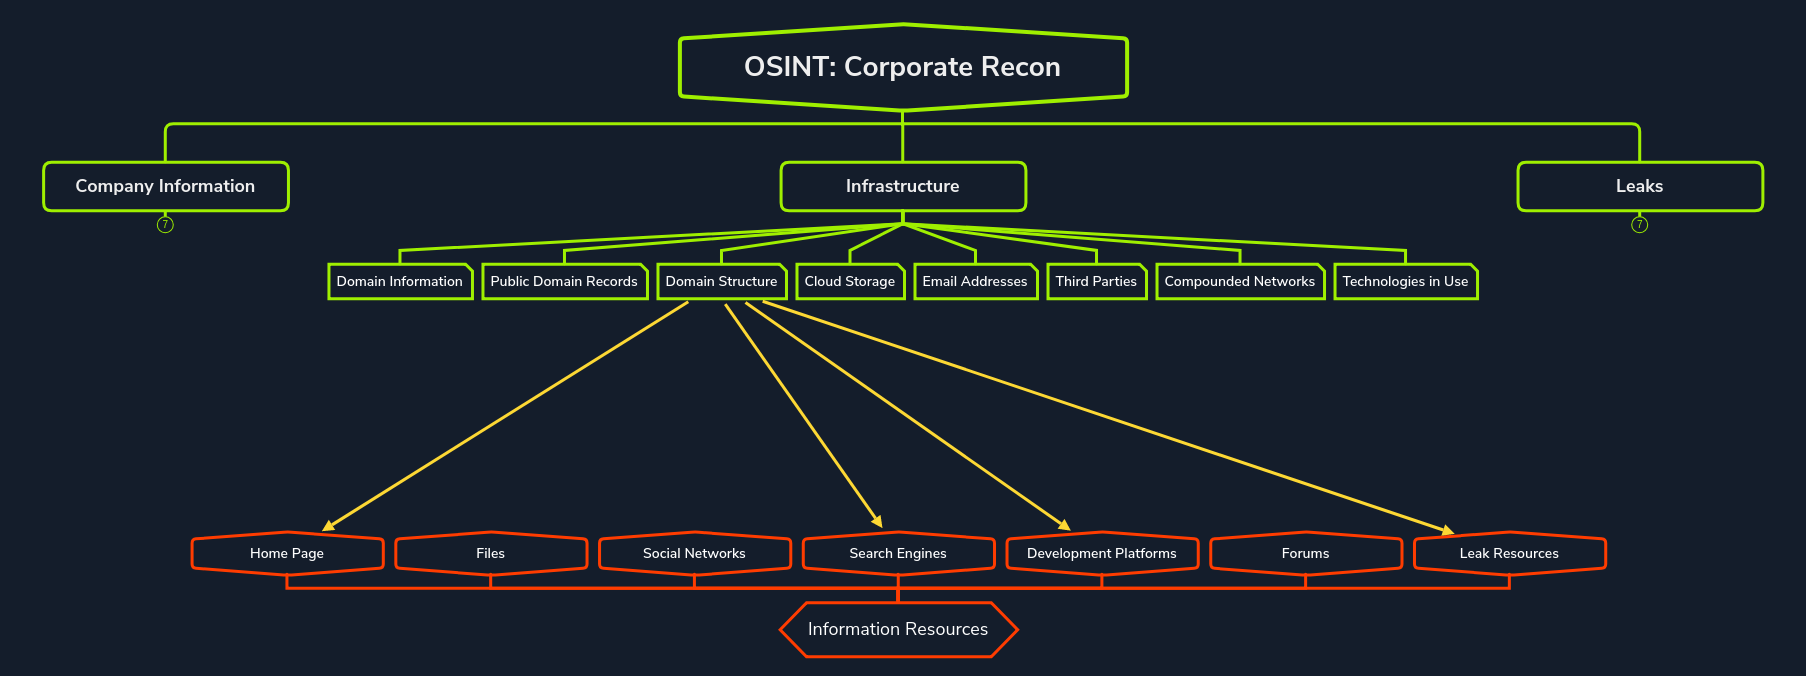
\includegraphics[width=\linewidth]{recon/osint/images/infra-domain-structure.png}
  \caption{OSINT Domain structures}
  \label{fig:osint-infra-domain-structure}
\end{figure}
This preparation can take several hours of study but save us time in the
following steps because we will not test each system blindly, but proceed
methodically, organized and structured. This represents the professionalism of
our work and gives a much better impression in the reports for our customers.

\subsubsection{Home Page}
Countless websites link to other subdomains. Therefore, we should always pay
attention to each clickable area on every web page owned by the company.

\subsubsection{Search Engines}

Since we are still in the passive information gathering phase, we should use
passive techniques to find out more subdomains. For this, we can use a tool
called \href{https://github.com/UnaPibaGeek/ctfr}{CTFR}. It uses Certificate
Transparency logs from
\href{https://www.certificate-transparency.org/}{Certificate Transparency} and
\href{https://crt.sh/}{crt.sh}.

\begin{verbatim}
./ctfr.py -d inlanefreight.com | grep -v "[-]"
\end{verbatim}

We can now use CTFR for each subdomain in a For-Loop because there may be other
subdomains in the respective subdomains. After we have collected and documented
all passive results, we can use a simple For-Loop in Bash to determine the
corresponding IP address for each subdomain.

Then we can use \verb+whois+ and \verb+ipcalc+ to find out the IP ranges for
the respective IPv4 addresses.


There are many different resources we can use to find out the IP addresses of
our target company. One of the best and most used resources is
\href{https://www.shodan.io/}{Shodan}. Shodan also offers a
\href{https://cli.shodan.io/}{CLI version} that we can install. This allows us
to query, filter, and save the results directly from the command line, making
documentation much more manageable.

\begin{verbatim}
shodan domain <TARGET-DOMAIN> |
    grep -w "A" | cut -d"A" -f2 | cut -d" " -f7 | sort -u > IPv4s.txt

for ip in $(cat IPv4s.txt);do shodan host $ip;done
\end{verbatim}

After this, we can use \href{https://ipinfo.io/}{IPinfo.io}. This resource
provides an excellent way to 
identify the subnets and hosting providers. Furthermore, we can use Spyse to
search for additional subdomains by entering the top and second-level domains
(e.g., target-company.htb).

Another great way to quickly search for subdomains is
\href{https://subdomainfinder.c99.nl/index.php}{C99.nl}. We should remember
that we should always use multiple sources to find all subdomains if possible.
This is because we will rarely have situations where a single source provides
us with all available subdomains.


With the IP addresses and subdomains, we can determine how many and which
subdomains are {\bf virtual hosts}. Some good sources that we can use are
\href{https://pentest-tools.com/information-gathering/find-virtual-hosts}{Pentester-Tools}
and \href{https://hackertarget.com/}{Hacker-Target}.
With the IP addresses and subdomains, we can determine how many and which
subdomains are virtual hosts (vHosts). Some good sources that we can use are
Pentester-Tools and Hacker-Target.

\subsubsection{Development Platforms}
or the developer platforms, we should be on the lookout for all possible files,
as eventually, any of them may contain hints about domain names or IP
addresses. Configuration files are of particular interest, as they may contain
access data and have fixed IP addresses and (sub)domains. For this, we can
again use \href{https://searchcode.com/}{Searchcode} to find files of this kind
quickly.

Another very interesting source of information is the
\href{https://www.seoptimer.com/}{SEOptimer}. This is an SEO analysis tool that
examines and evaluates the entire website for individual components.In general,
marketing tools are designed to evaluate visitors' interactions on the website
and allow SEO specialists and web designers to make the appropriate adjustments
to improve the rating or create a better UX. Since they work a lot with links,
we will likely find out a lot of helpful information.

\subsubsection{Leak Resources}

Leak resources are unauthorized publications of information. This term is broad
and can therefore include many different information components. These
resources also include databases with datasets containing information about our
target company. At the end of 2017, Rapid7 started
\href{https://opendata.rapid7.com/sonar.fdns_v2/}{Project Sonar}, which
collects and stores responses forwarding DNS requests. DNS records such as A,
AAAA, CNAME, and TXT lookups are stored at certain intervals in individual GZIP
files in the form of JSON. These databases are extensive and can exceed 30GB in
compressed format. They contain (sub)domains, record types, and the
corresponding IP addresses. This information resource serves as an updated and
valuable resource for us to understand our target company's domain better.

\subsection{Cloud storage}

\begin{figure}
  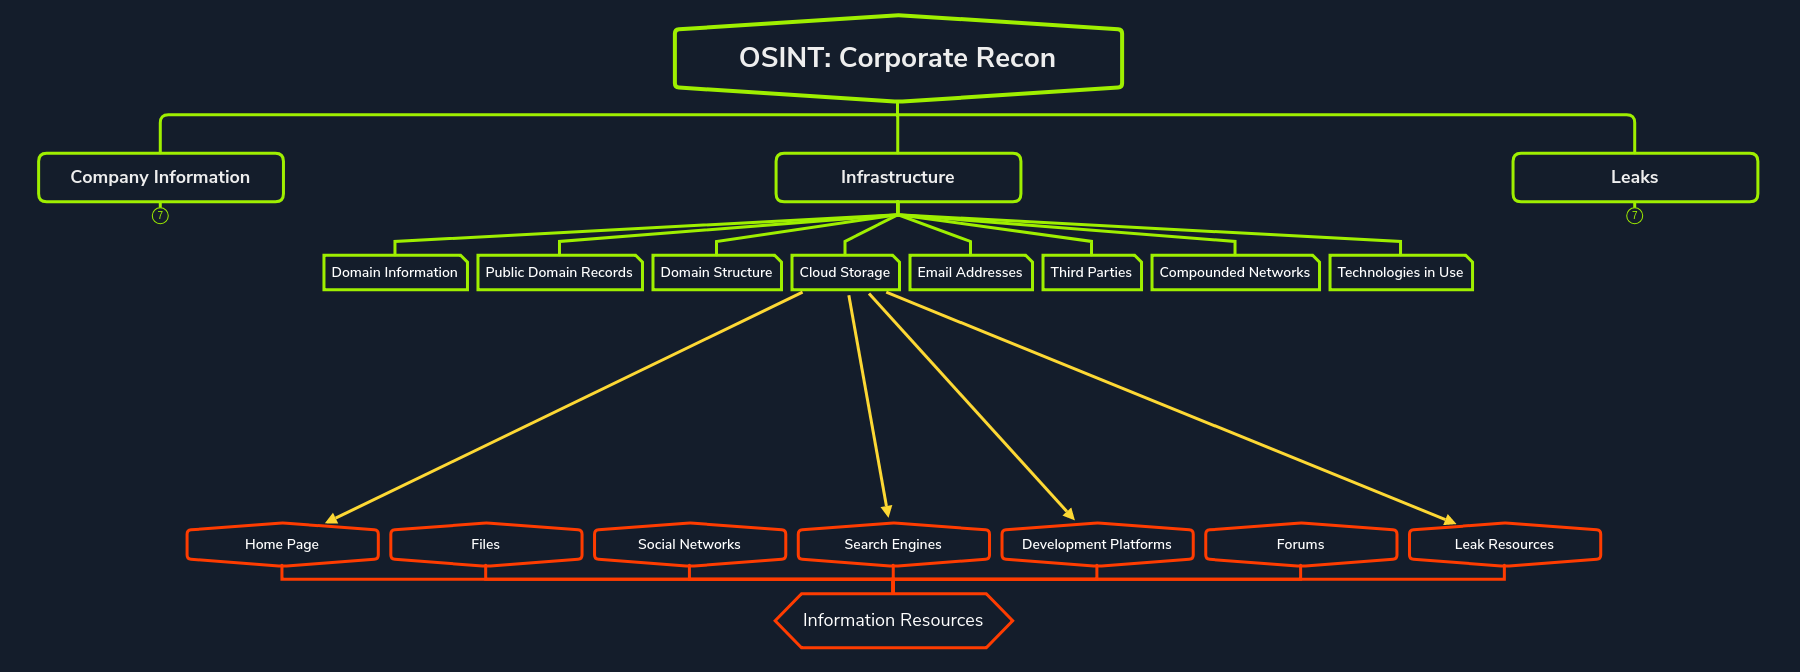
\includegraphics[width=\linewidth]{recon/osint/images/infra-cloud.png}
  \caption{OSINT Infra cloud}
  \label{fig:osint-infra-cloud}
\end{figure}

We can now resolve the domains found into IP addresses and compare them to the
netblocks for these three cloud providers. If we find any IP addresses within
these IP ranges, we can assume that it is a cloud provider. For us, the most
critical component in the corporate use of a cloud provider is open cloud
storage because if they have been misconfigured, they are publicly accessible
and viewable. Some of those cloud providers are, but not limited to:
\begin{verbatim}
 				
Cloud Provider 	    GCP 	                Azure 	    AWS 	    DigitalOcean
Open Cloud Storage 	Google Storage Bucket 	Block Blob 	S3 Buckets 	Spaces
\end{verbatim}

We can also automate this process with the tool
\href{https://github.com/oldrho/ip2provider}{ip2provider.py}. This will
automatically compare the IP addresses with the netblocks and show if they are
successful matches.

\begin{verbatim}
cat Target_Company.IPv4s | ./ip2provider.py
\end{verbatim}

\subsubsection{Home Page}
When searching for cloud buckets, one factor makes it difficult for us to
identify the bucket belonging to the company. This is that everyone can create
their own name for the desired bucket. This means that anyone can create a
bucket with the target company's name without it belonging to the company.

Here we can also find a list of URLs from which we can see which cloud provider
the storage belongs to and where we could find it.

\begin{verbatim}
Cloud Provider 	URL
GCP 	https://www.googleapis.com/storage/v1/b/<bucket-name>/iam

Azure 	https://<bucket-name>.core.windows.net/<container>/
	i   https://<bucket-name>.blob.core.windows.net/<container>/

AWS 	https://<bucket-name>.s3.amazonaws.com
	    https://s3-<region>.amazonaws.com/<company-name>
\end{verbatim}

Almost all (~95\%) vulnerabilities in the cloud happen due to misconfigurations. These misconfigurations include, but are not limited to:
\begin{itemize}
    \item   ACLs
    \item   Bucket Policies
    \item   Service Control Policies
    \item   Public Access Blocks
    \item   IAM Policies
\end{itemize}

Cloud environments extend the penetration testing process enormously. However,
this does not affect the OSINT process since we ultimately use public resources
to not interact with our target company. Further investigation of cloud buckets
will be covered in another Module, as we need to investigate and understand the
setup and the individual configuration options to work with them effectively.
However, we already know enough to find open cloud buckets. Whether they are
open and whether we can see the content on them requires interaction.
Therefore, we will stop after finding them, and in the next stage, we will deal
with them and enumerate them.


The first information resource often used for this purpose is the company's
website. Buckets are often used as a source for the web servers and their
contents are linked accordingly.

We can also use this content and the names of the files or the company's full
domain name (i.e., www-target-company-com) for Searchcode to see if they are
publicly retrievable and if there might even be more information resources for
them. To do this, we take the name of the file and can, for example, look for
other cloud providers to see if they are available there. The more unique the
name of the file is, the more accurate the results will be. These are then
easier to identify and connect to the target company.

\subsubsection{Search Engines}
If files have been tagged or named in conjunction with the company name, we can
use the search engines we know and filter the results based on the cloud
providers. Aside from file names and company names, we may also use employee
names or application names if they appear unique. For this, we can set the
known domains from the cloud providers as the assumed content (with the
\verb+inurl:+ tag) for our results. This will reduce the results only to those
that contain this domain. Finally, we know that the buckets' label will not
necessarily have the name or label we have already seen. For this, search
engines help us to expand our search scope but also to reduce it.

Another information resource that serves very well for finding such buckets is
the \href{https://buckets.grayhatwarfare.com/}{GrayHatWarfare Project}. This
project is an online tool that searches for open cloud buckets and archives
them. This is one of the most widely used tools currently, and it also gives
excellent results since it contains an enormous amount of records.

The GrayHatWarfare Project offers us many different options, such as filtering
by buckets, files, file types, keywords, and even an API interface. We can
search these buckets for files and see which of them might be relevant for us.
The advantage is that we do not have any interaction with buckets owned by the
target company as long as we do not explicitly call the files or list them via
the CLI.

\subsubsection{Development Platforms}

Again, developer platforms are of great use to us, as we can search code to
find out if specific files exist in connection with the cloud buckets. As we
know, {\bf Searchcode} also redirects us to the resource that points to the
corresponding file. Often used strings in these files are {\bf AccountName} and
{\bf AccountKey}, used for authorization (like username and password).

These files usually contain the {\bf IP addresses} or the {\bf bucket names} for the
corresponding cloud storage. We can use these to search again on {\bf
GrayHatWarfare}
and filter out the results. Therefore, if we follow these files and examine
them more closely, we will most likely find a lot more helpful information that
we will need for our documentation and further research. 

\subsubsection{Leak Resources}

Another source that can point us to the buckets and forward them is the
aforementioned \href{https://opendata.rapid7.com/sonar.fdns_v2/}{Rapid7
database}. Since this works with the forward DNS requests and responses and
documents those, it is even very likely that we will find entries that will
show us the corresponding buckets.


\subsection{Email Addresses}
Identifying existing email addresses can also provide us with a massive attack
vector that we can use to our advantage. We can use emails in many ways. Among
other things, email can be used not only for phishing attacks, but we can also
analyze the traffic of these to identify which is the "central" point for the
processing of emails. After all, this will have by far the most sent emails. We
can also subscribe to newsletters and analyze their headers with MXTools, which
will also show us the route of the email and its security settings.

\begin{figure}
  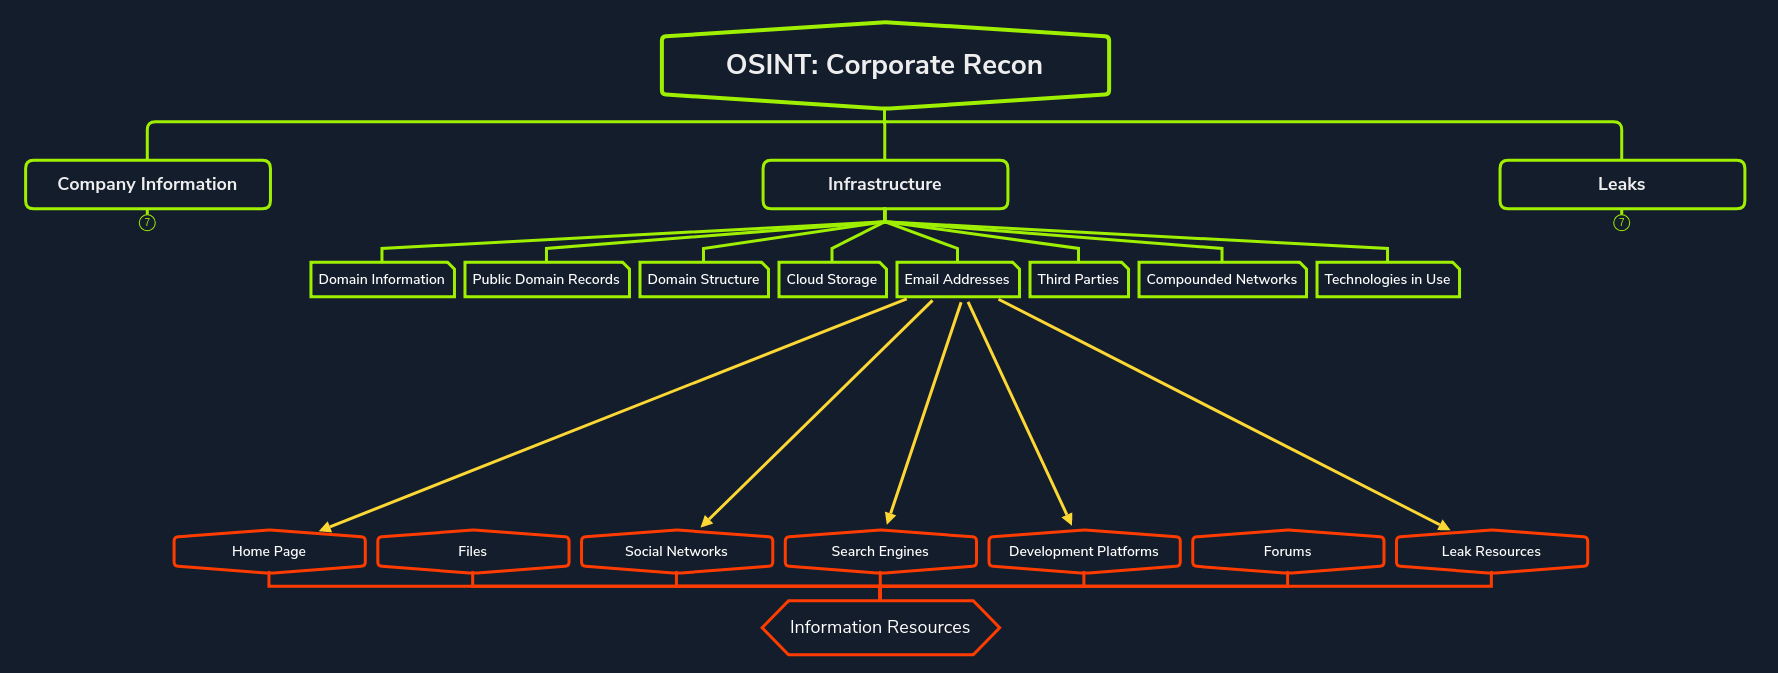
\includegraphics[width=\linewidth]{recon/osint/images/infra-emails.png}
  \caption{OSINT Infra Emails}
  \label{fig:osint-infra-emails}
\end{figure}
Email addresses may have different structures even within the same company. One
of the most common examples is when the first and last name
(first.lastname@domain.tld) is used in the email address. However, the email
addresses can be created with usernames (username@domain.tld) not to show the
user's full name.

\subsubsection{Home Page}

The company's website is often the stop for us to find out interesting
information. In most cases, we find the first points of contact through email
addresses on the contact or about page. We may find email addresses for
personal contact with the individual, for business and informational purposes,
as well as for job applications or even department heads. This also helps us to
understand very well how the internal infrastructure may be set up. In larger
companies with multiple locations, the individual departments are managed with
the country codes available in the email addresses. Therefore, we can often
find information on the offices or local information pages. It is helpful if
the individual departments and their functions are described on this page,
which can help us to understand the internal infrastructure better.

Finally, companies often try to use as short terms as possible, as these are
easier to remember and require less effort to type. Therefore, the domains for
the email addresses can be different but still belong to the same domain. For
example, if we find a company with the name Target-Company.com, the abbreviated
variant could be TarCom.com or TC.com, if they are still available.


\subsubsection{Social Networks}

As we already know, many conversations occur on social networks, and therefore
a lot of information is shared. We can also find email addresses there that
point to particular addresses for exceptional cases. Here we can use the
combination of social networks and search engines to find them. In the search
engines, such as Google, we then use the corresponding Google dorks
(\verb+inurl:+ and \verb+intext:+) to optimize social networks' results.


For the dork \verb+inurl:+ we set the domain of the corresponding social
network we are looking for. Next, we use the dork \verb+intext:+ with the
extension for an email address (\verb+@domain.tld+) that belongs to our target
company. This then gives us some results that we can further investigate to
establish further links.

Another critical role for email addresses is their {\bf reputation}. This could
tell us whether the corresponding email address has already been used for spam
activities, has been blacklisted, whether {\bf SPF} or {\bf DMARC} is used, and
much more. To get this information, we can use the information resource called
\href{https://emailrep.io/}{Emailrep}. Apart from the information we get from
it, using the API is very useful for us as we can easily use it with cURL.
\begin{verbatim}
curl -s emailrep.io/info@target-company.com
\end{verbatim}

It for example provide the information if the email is {\bf spoofable}


\subsubsection{Search Engines}

Once we have worked through the most used social networks, we can use the
search engines to look for other information resources, including company email
addresses. We can use the same Google Dork (\verb+intext:+) to filter the
results and match them with the existing list.

On the first page of the 18,000 results, we can already find an email interface
of the company based on this simple usage, which can and should also be
investigated in more detail later (if the scope allows this). Suppose we
encounter a case where a large number of results appear that belong to a single
domain. In that case, we can also use the dorks to exclude specific information
resources by placing a minus in front of the dork (\verb+-inurl:+).

A very efficient tool for this is called
\href{https://github.com/laramies/theHarvester}{theHarvester}~\ref{tool:theharvester}. This tool
    searches the information resources we provide, such as Google, Netcraft,
    Spyse, Twitter, and others for entries. Some of these services offer API
    keys that are bound to the corresponding account to execute the requests.
    Often there are limits on the number of requests we can send.
\begin{verbatim}
theHarvester.py -d inlanefreight.com -b google,hunter,netcraft,spyse,twitter,dnsdumpster
\end{verbatim}


\subsubsection{Development Platforms}

Apart from insight into the company's technologies and source code, development
platforms also serve very well to find out email addresses. Developers' email
addresses are interesting, as they are often linked on different platforms,
which we can then investigate and analyze later in the staff investigation
phase. We will go into this in another Module called {\bf OSINT: Staff
Investigation}.

Here we can also use the combination of the developer platforms and the search
engines to find out the developers' email addresses. Just as we used the Google
Dorks for social networks, we use them again, only this time for the developer
platforms.

Another useful combination is searching for images in connection with the email
addresses. This search option is usually overlooked, as most people do not see
any relationship between email addresses and images. However, users often
upload images linked to such an email address in the text or in some other
way.

A small difference is that we no longer use the \verb+inurl:+ dork for the
information resource but \verb+intext:+ to extend the linking to the individual
information resources.

\subsubsection{Leak Resources}

In principle, leaks can be displayed in any form. What counts is how, where,
and what exactly was found. It becomes much more relevant when this information
is used to complete and adapt an attack against the company. Here, the attitude
of the developers to the information they discuss in public plays a significant
role. Moreover, some are unaware that the information they share can be viewed
publicly, assuming no one is looking for it. Furthermore, it is precisely this
kind of attitude that often puts companies at risk of being attacked.


Moreover, several factors come together because even if the developers are
aware of it, misconfigurations are another factor that makes even their
settings seem ineffective. Misconfigurations can even lead to calendars with
appointments being publicly visible.

Email addresses often play a significant role in this field, as they are linked
via a wide variety of platforms. Let us consider that passwords are often used
repeatedly across multiple platforms. The risk is relatively high that if we
can find a password for an email address and log it into a company's email
interface, this will lead to significant information leakage that may even
result in full compromise. One of the most effective tools that can be used to
support linking is \href{https://github.com/khast3x/h8mail}{h8mail}.

\begin{verbatim}
8mail -c h8mail_config.ini -t first.lastname@target-company.com
\end{verbatim}

From the results, we can see that the email address we analyzed is contained in
seven different databases whose passwords can be viewed. Another option is to
use the service of \href{https://haveibeenpwned.com/}{HaveIBeenPwned} to
determine if any of the email addresses we found are already in databases that
contain passwords for them and have been compromised.

HaveIBeenPwned also goes through all available databases and checks the entries
for the existence of the email address we entered. It will show us which
platforms have been affected by this data's loss if it is there.

\subsection{Third Parties}
Identifying third-party providers requires a little more manual work and
research. Since we know that there may be severe legal consequences for us,
including a criminal charge, we should look at this issue here. In the case of
a black-box penetration test, we must pay close attention to which third-party
providers offer services to our target company.

However, this does not mean that we are not allowed to test systems from
third-party suppliers. For this purpose, "Penetration Testing Authorisation
Forms" exist, which must be filled in and submitted. This is to inform the
third-party vendors that they will most likely receive alerts for the specific
systems and should be aware that this is done with our intent. This will also
prevent our Internet Service Provider (ISP) from being contacted and blocking
our access to the internet. It will also stop us from being charged for
attacking the hosts.

We should not use attacks such as DDOS unless all parties have agreed to do so
not to restrict the services we provide to other users. But here, too, there
are always precise specifications (Penetration Testing Rules of Engagement)
from third-party suppliers that we have to follow.

If no forms are available from the third-party provider, our customer must
contact the third-party provider and obtain permission. Otherwise, our customer
must fill out and submit the documents and provide us with confirmation of
permission to test the systems.

\begin{itemize}
    \item Amazon Web Services
        \url{https://aws.amazon.com/forms/penetration-testing-request}
    \item Digital Ocean
        \url{https://cloud.digitalocean.com/support/tickets/new}
    \item Google Cloud 	\url{https://support.google.com/cloud/answer/6262505?hl=en}
    \item Microsoft Azure
        \url{https://security-forms.azure.com/penetration-testing}
\end{itemize}

By now, we should have gathered enough information to keep an eye out for the
third parties. When looking for them, we must assemble an extensive collection
of information resources.

\begin{figure}
  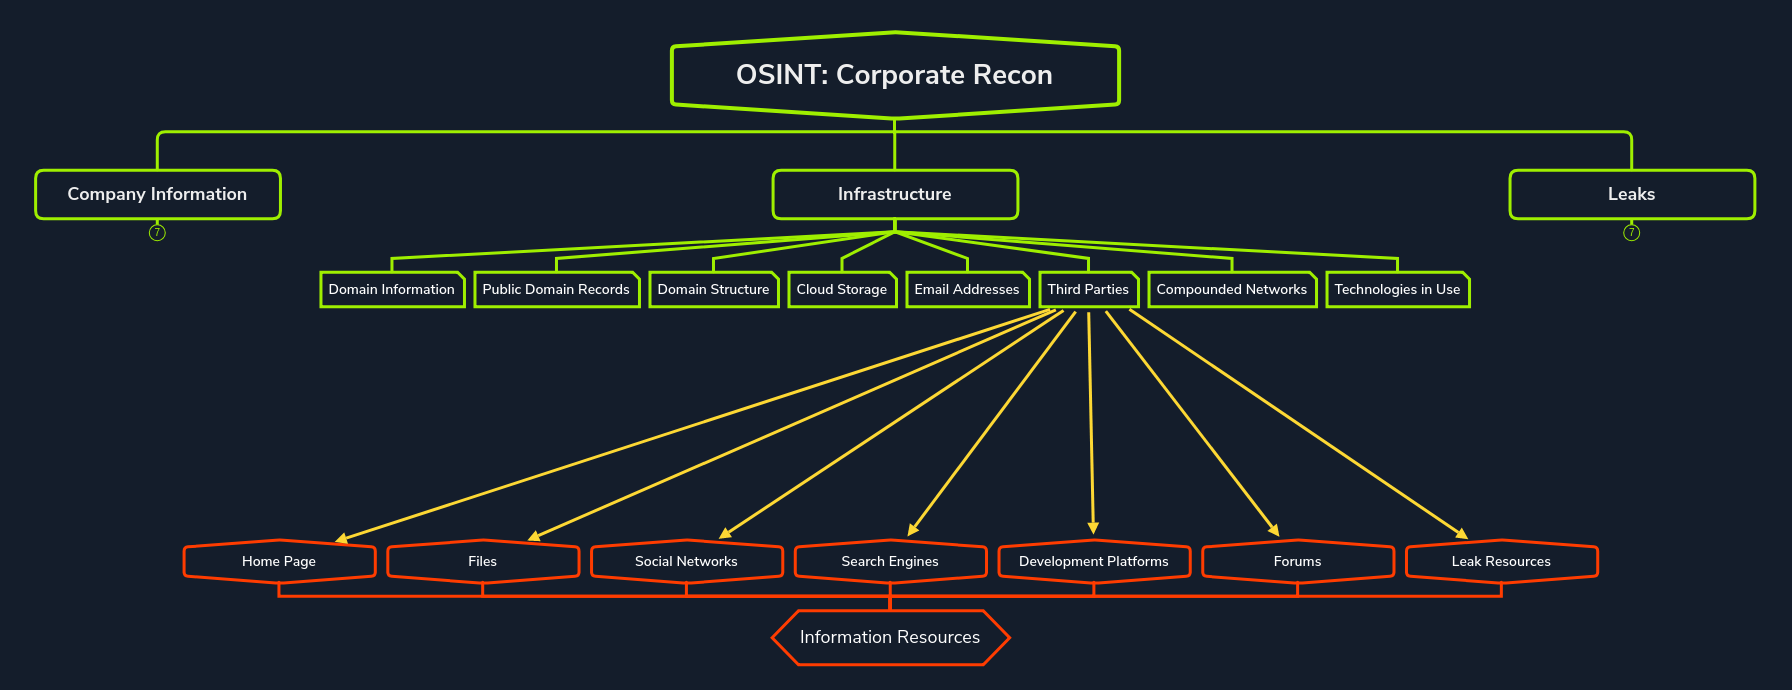
\includegraphics[width=\linewidth]{recon/osint/images/infra-3rd-parties.png}
  \caption{OSINT Infra third parties}
  \label{fig:osint-infra-3rd-parties}
\end{figure}

We can see from the graph that we can get this information about third-party
vendors from pretty much any information resource. We will go through the
information resources that we have transferred to our Resource Browser in this
step. If we have followed the methodology, we already have many information
resources such as different websites, providers, files, and images that we can
use for this. Here we need to summarize them and get an overview of how the
company is positioned and which providers are used.

Apart from the different software the company uses, the hosting providers play
an essential role. Based on this, we will assess how extensive the inventory is
in the cloud, if at all, and what these {\bf hosting providers} offer for
security measures.


\subsubsection{Hosting Provider}

It is always necessary to establish who the third-party providers are and what
services they provide to the company. This should always be discussed in the
meetings before the penetration test.

\href{https://securitytrails.com/}{SecurityTrails} does an excellent job in
this research, which we should take advantage of.

Based on these results, we determined the four different hosting providers that
our target company uses. We can search for the names of the hosting providers
on Google, for example, and see their penetration test policies and rules of
engagement and how best to get permissions for them.

If we do not find a hosting provider in the list, it is most likely a
self-hosted system.

\subsubsection{Documents}

Here we should take a closer look at the providers who could make files
available to us. These files can contain valuable information about the company
itself and its processes and show us whom they work with to manage the
infrastructure. For this search, we use the search engines like Google with the
dork \verb+site:+ which will limit our searches to the pages we need. The most
used providers for documents include, but are not limited to:

\begin{verbatim}
Google Docs 	        site:docs.google.com
Google Cloud 	        site:cloud.google.com
Google Storage 	        site:storage.googleapis.com
Microsoft 	            site:docs.microsoft.com
Amazon Web Services 	site:amazonaws.com
\end{verbatim}


\subsection{Compounded Networks}

Compounded networks use platforms that are suitable for both {\bf personal} and
{\bf business} purposes. The difference between information sharing and
information dissemination is that people on these platforms disclose less
information about themselves. They want to make sure that potential employers
or their current employers do not get the wrong impression. Confrontation is an
essential aspect of professional life that every employee wants to avoid.

\begin{figure}
  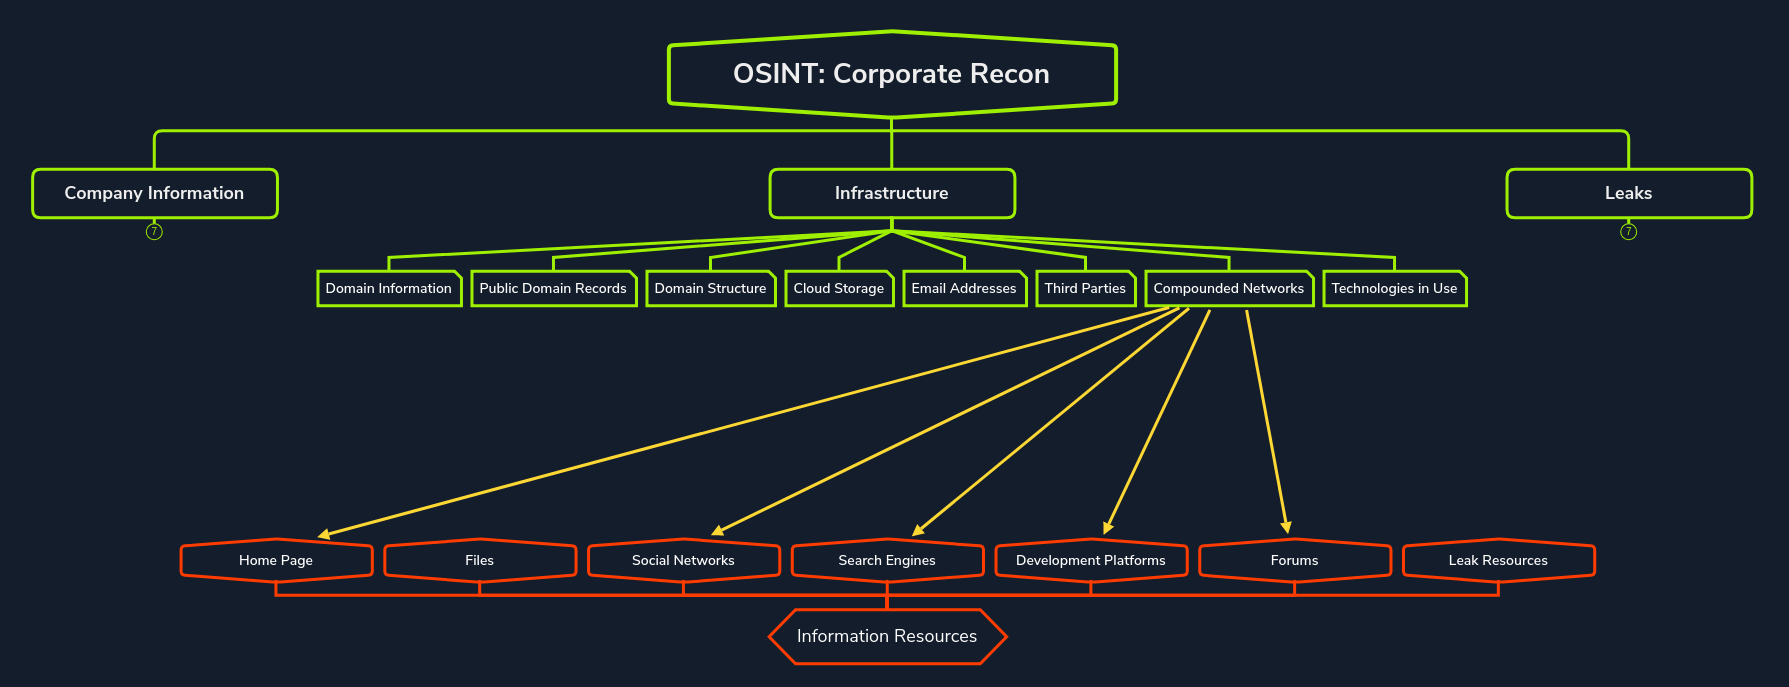
\includegraphics[width=\linewidth]{recon/osint/images/infra-networks.png}
  \caption{OSINT Infra Compounded Networks}
  \label{fig:osint-infra-networks}
\end{figure}
In most cases, we can already find all the links to the social networks on
which the company is linked on the company's home page. The best known
compounded social media platforms are, but not limited to: Facebook, Instagram,
Twitter

Another essential difference between real conversations and opinions on social
media platforms is that people often express views on a topic that they would
not usually have the courage to communicate in a face-to-face conversation.
This is because people feel safe to express their opinions at a distance
without the risk of provoking direct conflict, and above all, they have much
more time to respond than in a face-to-face conversation.

By reading through such comments and posts, we can create a pattern of how our
target employee thinks about a specific topic. Above all, security-relevant
information may be published when one is actually looking for help. However,
the stress and worry that we get careless and unfocused can lead to such
publications of security-related information.

Furthermore, posts on these platforms can also draw attention to illegal
activities by the employee. Suppose our employee, as an example, has taken
specific courses and training paid for by our client, and the employee shares
this publicly with all others. In that case, it is a violation of the general
terms and conditions for which our client is liable and accordingly also
security-relevant. We cannot say whether company-specific information has been
shared, but we should investigate the employee more in detail to prove or
disprove this fact.

\subsubsection{Social Networks}

Here we focus not on the search for compounded social networks but the content
within them. For this purpose, the corresponding {\bf hashtags} are suitable,
which primarily connect users with the company. In addition to the individual
persons, partners can also be recognized, since they often thank them for a
friendly comment or can also make themselves known through some other
activity.

The focus here is on finding social groups created either by the company
itself, its employees, or third parties in which specific topics are discussed.
In doing so, we should narrow down the search for these groups as best we can
with the information we have already obtained. After all, if we search only for
Java, we will get quite a few results that will make our work more difficult.
However, if we use several terms, such as \verb+Java + target-company + web
interface+, we will reduce our search results many times and become much more
precise.

Basically, in compounded social networks, we can obtain internal information
that is not directly visible. To do this, we should examine fields such as
groups, comments, images, and the like. It is crucial to trace the entire
conversation as best as possible and try to find out the background and why and
how it came about that this conversation is taking place. Complaints that
reflect employees' internal impressions of the company are excellent indicators
of this.

\subsection{Technologies in Use}

One of the most valuable pieces of information about the infrastructure is the
technologies the company uses. Often it is not always easy to get much of this
information passively. However, we do have some tools at our disposal to help
us extract this information. Here, too, any information resource can be of
great importance. The focus here is on identifying technologies that we can
later use to adapt our attacks against the company. Especially for social
engineering attacks, this plays an important role later on. We can interact
with the employees and communicate and build trust with customized information
(which only trusted people know).

\begin{figure}
  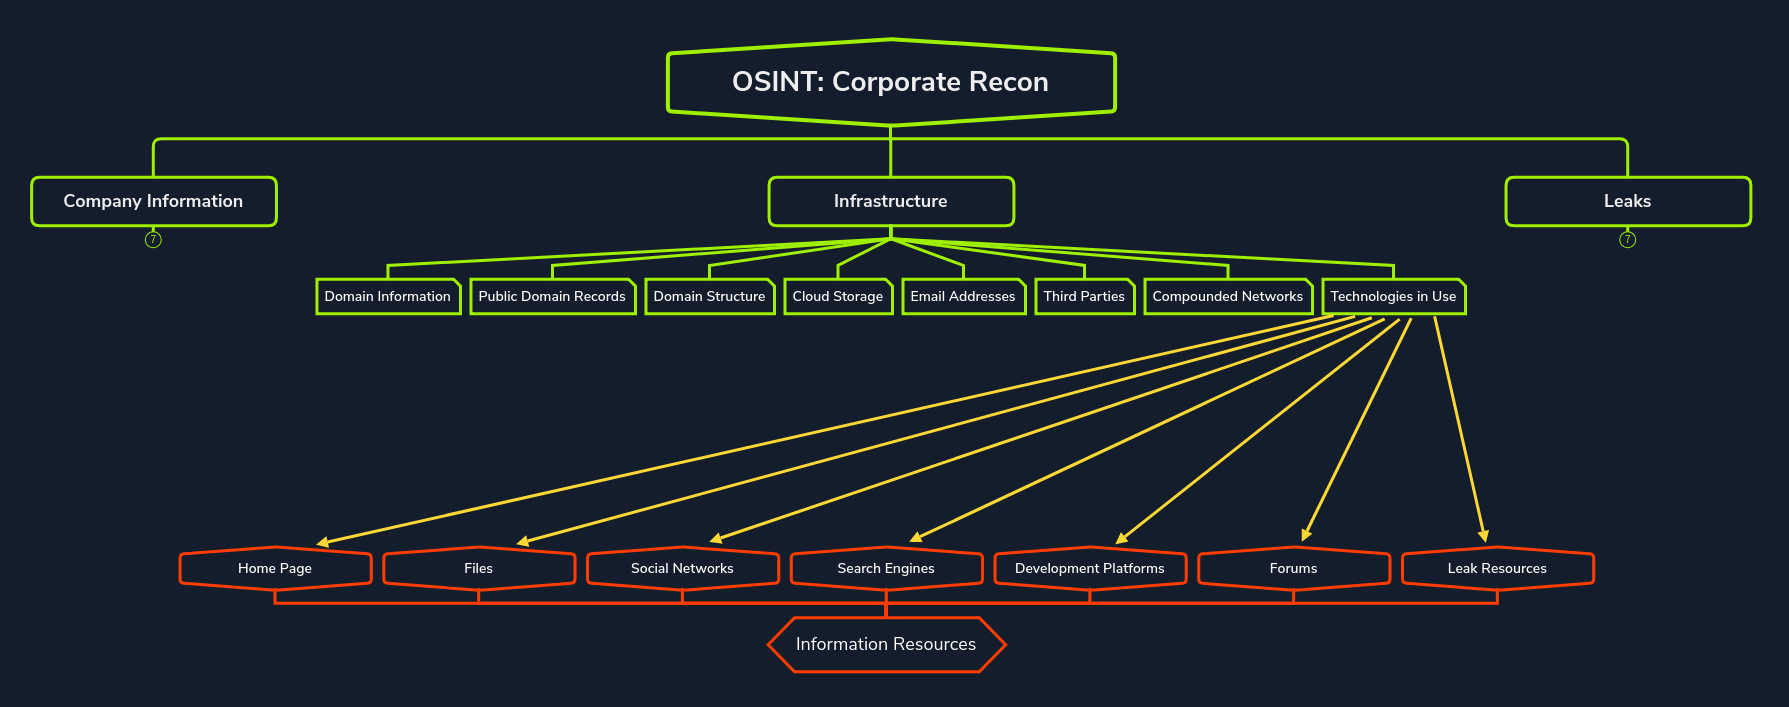
\includegraphics[width=\linewidth]{recon/osint/images/infra-techs.png}
  \caption{OSINT Infra Technologies}
  \label{fig:osint-infra-techs}
\end{figure}
Such information includes any software or provider that makes such an
application available. Once we understand what the company is using
technologies, this will give us a reasonably accurate picture of the aspects
that will be most relevant to us as we prepare our attack on the company.


\subsubsection{Home Page}

We can already learn a lot of information from a company's home page. This can
be, for example, different forms or content from the source code of the page.
Especially with CMS, like WordPress applications, it is quite helpful because
they are individually combined with different plugins. Often, weak points are
found in the individual plugins, which can then be exploited to penetrate the
company's network.

Another beneficial source that can tell us a lot about the target company's
website alone is \href{https://builtwith.com/}{BuiltWith}. It lists all the
technologies that are used by the web server and are deployed on it.

BuiltWith analyzes the content of the website and identifies the technologies
used for it. This gives us an even better overview of how the web developers
work and their knowledge, which we can use to assess how experienced they are.
This is because we can use our assessments to identify or rule out certain
security-related aspects, making our attack vector much more straightforward.

\subsubsection{Search Engines}

In the section Public Domain Records, we already used the Shodan CLI to find
information about the respective IP addresses. Shodan showed us which services
it recognized and the technologies behind them. We can get the necessary
information about the domain from Shodan using the "domain" parameter and see
what details we will find about it. Most of the time, we get a good insight
into the systems related to the domain, and sometimes we can even identify the
vhosts directly, apart from the subdomains. Sometimes we can even find other
domains with different TLDs that extend our attack vector if the scope in the
contract allows it.
\begin{verbatim}
shodan domain target-company.com
\end{verbatim}

hodan also has databases in which information is stored over a specific and
relatively long period. We can use the Shodan CLI to search this database for
entries related to our target company.

\begin{verbatim}
shodan search target-company | cut -d" " -f1-3
\end{verbatim}

\section{Leaks}
We can use the same techniques we have learned so far for leaked information.
However, the focus here is on information that only employees are likely to
have. The word "leak" refers to a source of leakage in companies,
organizations, and governments. In this case, information is disclosed that is
not intended for public consumption. This information can still be damaging,
regardless of the company's infrastructure.
\begin{figure}
  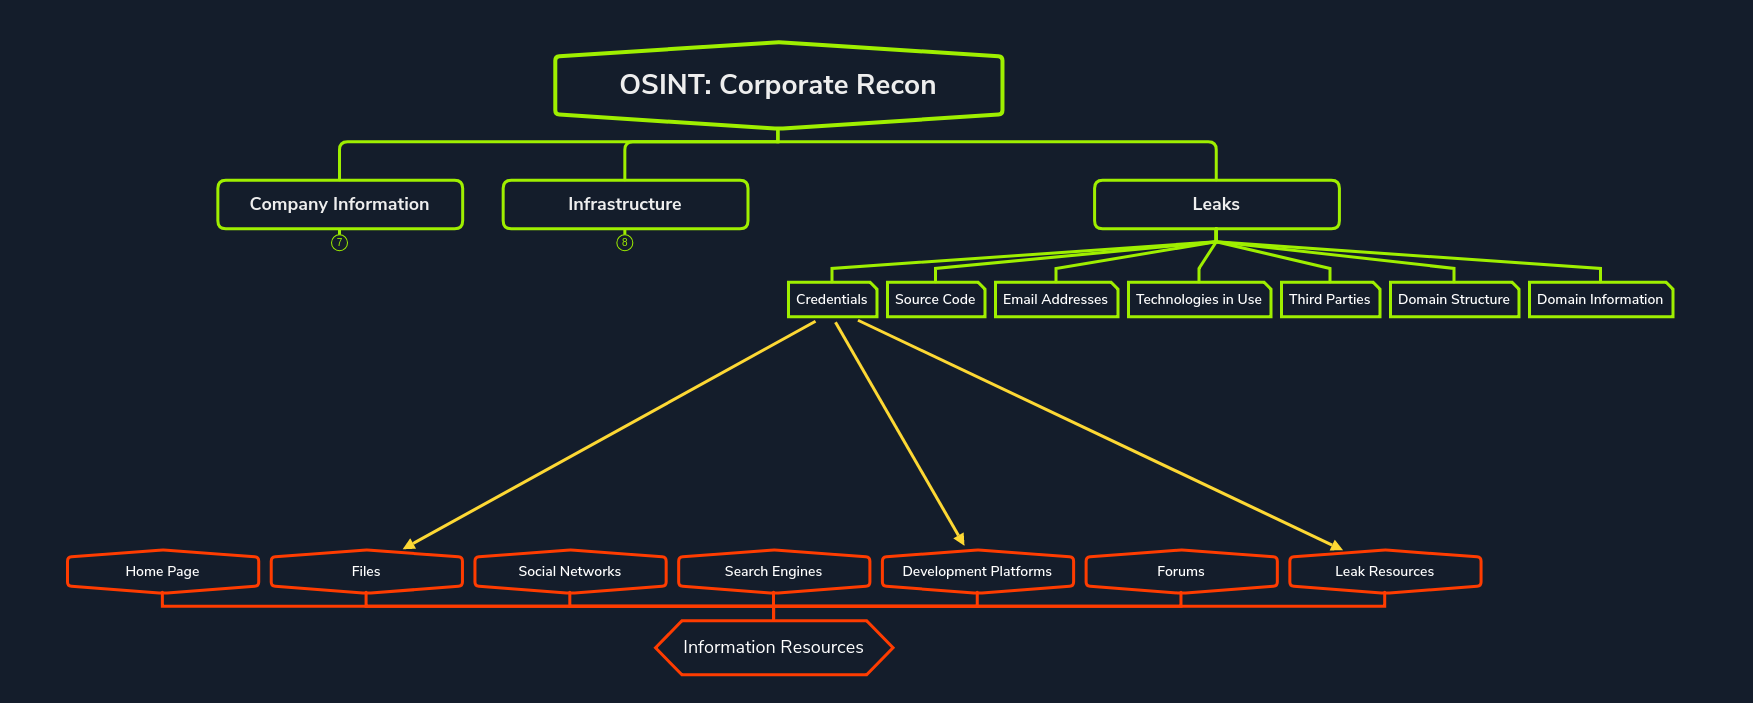
\includegraphics[width=\linewidth]{recon/osint/images/leaks.png}
  \caption{OSINT Leaks}
  \label{fig:osint-leaks}
\end{figure}
Leaks are not only made by attackers but also by the company's own employees.
If it is an employee, the cause of such information disclosure can be either
{\bf accidental} (through carelessness), {\bf intentional}, or {\bf forced}. In
the third case, it is a lose-lose situation into which one has been forced and
in which there is usually time pressure.

{\bf Accidental leaks} represent a disclosure of information and data that, in
most cases, is intended for internal purposes only. This is done only by the
employees of the company for many reasons. Generally, accidental leaks are
referred to as {\bf information disclosure}.

To illustrate this as thoroughly as possible, we can imagine source code that
contains commented-out credentials that the developers have inserted for
convenience. Suppose, however, and we find these credentials in the source
code, which is an essential part of its function. In that case, it is
information disclosure and no longer refers to the contents of the code but
access rights (and thus to the administration and configuration of the
system).


{\bf Intentional leak} takes place purposefully and always has the goal of
making secret, confidential or private data public. With a leak, an insider
wants to expose dishonorable, immoral, unethical behavior and make it
accessible to the public. In some cases, attackers want to cause damage with a
leak.

If we go back to our previous example and assume the developer added those
credentials there on purpose and the intent for harm, then this is a leak.

In a leak, rules and laws are deliberately broken. Because at its core, a leak
is data theft and violates confidentiality agreements. A leak becomes possible
when an internal employee violates the trust and security rules given to them.
For attackers, a leak requires them to find software vulnerabilities to steal
data. A leak can occur by an insider who had legitimate access to the data, but
it does not have to. Websites or social media profiles can also be hacked by
outsiders, allowing data to be stolen. The insider, also known as a
whistleblower, remains anonymous to avoid prosecution.


A {\bf forced leak} means that the person or organization concerned often has
no way to avoid the prospective personal or cooperative damage. This type of
disclosure usually involves blackmailing the person or organization concerned.
This is often the modus operandi of various malware activities that force the
person or organization to pay with money or specific activities, or the
encrypted/stolen data is kept and published. These are cases where {\bf Digital
Forensics and Incident Response (DFIR)} is used to identify the attackers and
undo the damage caused by the malware.

The source of a leak can be any conceivable information resource. We can see
how efficient our methodology is since we no longer base our information
gathering approach on information resources but on the categories of
information we want. Here we examine the information resources already found
for the data for each category. There are information resources designed to
find this type of content, and these are divided into three fields, {\bf
archives}, {\bf internal leaks}, and {\bf breaches}.

\subsection{Archives}

An archive represents anything that contains an enormous amount of written
information in some structured form and is not a library. It is therefore used
to store information that can be accessed (un)restricted. An archive,
therefore, stores information about the required information resource at
specific intervals with special conditions. From 1999, it has been extended by
other archives, so it is now a digital library that includes significant
collections of texts and books, audio files, videos, images, and software. The
Internet Archive is dedicated to the long-term archiving of digital data in a
freely accessible form.

Besides the already mentioned forums and social media platforms, archives
should not be left out. These archives, such as
\href{https://archive.org/}{WayBack Machine} or
\href{http://archive.fo/}{Archive.fo}, create so-called snapshots or captures
of websites and store images, videos, audio recordings, software, and files
that have been published on the websites.

These captures of web pages are taken by a crawler. In 2018 the WayBack Machine
archived over 380 billions of web pages. Viewing older versions of these sites
also allows us to see and analyze the source code. This can include, for
example, the robots.txt of a web server, which may indicate hidden folders on
the webserver that still exist.

We can also display URLs that the WayBack Machine has crawled. Here it is often
shocking how many URLs are publicly accessible even if we think that the
published information from the past no longer exists. We may also find content
that has been removed by our target company for security reasons, for example,
that describes their technology in too much detail or even reveals other
information such as their internal processes.

Another interesting feature of WayBack Machine is that it also shows us in the
Summary how many new links it has captured compared to the previous year. Here
we get an overview of potentially existing folders and files that are now
hidden from the public but still exist for further development or as a backup
on the system. These can be detected using the filter located at the top right
above the table. There we can enter the file extensions that are being searched
for. Applications and administrators use many different file extensions. A list
of them can be found at
\href{https://fileinfo.com/filetypes/backup}{FileInfo.com}.


Another critical information resource is
\href{https://pastebin.com/}{Pastebin.com}. There, different people share
information in text form with each other. Pastebin is a web application that
acts as a kind of online clipboard and can store any text, even large text
blocks, on the web and make it accessible to third parties via a link. The
interesting feature of the tool is that it supports syntax highlighting for
many programming languages. This makes the code much more convenient to read
and easier to understand. Since this feature, which is crucial for programmers,
is missing from most blogs, social networks, forums, or chat programs, it has
been reported that there are now over 15 million "pastes" on the website.
Pastebin now offers some options not to save the shared information
permanently. These include setting a password, which in most cases are
relatively weak, and the Burn after reading function, which deletes the content
after viewing. As we have done in previous search engine searches, we can also
narrow down the results using the \verb+site:+ dork to the Pastebin page, giving us
some impressive results.

\begin{verbatim}
site:pastebin.com XXX password router
\end{verbatim}

he art of finding this type of information is to combine the different
information that we already know. To efficiently discover these leaks, the
research we have done in the previous sections is necessary. Otherwise, we
would be blindly searching for leaks on the off chance that our search might
take an incalculably long time and even yield no results.

\subsubsection{Internal Leaks}
Most employees who create and edit documents and are not familiar with IT
security may not know which data will be published even under certain
conditions. They are cautious about what they write in the document. Still,
they don't know that it is not always necessary to write sensitive data in the
documents, whether it contains information about the company's working
environment.

Almost all websites have their own images, files, documents, and notes which
they make available to the visitors. In most cases, these were created or at
least edited on computers. Whenever files are modified, so-called metadata is
written to the resulting files. These often contain the name of the application
that was used for it and sometimes its version. Even some operating systems
write their own metadata into these files.

For a regular user, this data is irrelevant. Still, it gives us an excellent
insight into the employees' working environment and the software they are using
along with the versions.

One of the most effective and most comfortable to use tools is Exiftool. On the
website of our target company, we could find some reports which are available
for download. We can take advantage of them, download them, and examine these
reports to determine if specific metadata has been added to the files.
\begin{verbatim}
exiftool document.pdf
\end{verbatim}

We already know which software and version were used to create this document
from the downloaded document without looking at its contents. We also see
precisely when this document was created and last edited. We can also see the
PDF version, encryption type, language, operating system used to create this
document, and other valuable information.

Since we know that specific software tends to insert its metadata into files,
we must be careful how we download the files from our target company. Often,
when we download images using Firefox, we can see that the metadata, such as
the date and time of creation, may differ from actual values. It is therefore
recommended to download these files via wget to avoid accidentally manipulating
the metadata.

Internal leaks include almost any file from which we can extract metadata.
However, other sources may reveal internal information. The more we analyze the
company, the better we learn to understand its structure. This gives us a
variety of results, which can lead to internal calendars.

Calendars contain not only the date and time of certain events, but also names,
email addresses, locations, topic content, links, and other information. This
makes them very valuable, as it is assumed that no third party can access this
information.

Not only metadata and poorly hidden internal applications can provide us with
valuable information but also whole software or code published on
\href{https://github.com/}{Github} or \href{https://gitlab.com/}{Gitlab}. This
content can also contain security-related information that developers have
forgotten to remove.

\subsubsection{Breaches}

When we talk about breaches, we mean any documentation of existing losses of
information. Apart from various news like the attack on
\href{https://www.cnet.com/news/solarwinds-hack-officially-blamed-on-russia-what-you-need-to-know/}{SolarWinds},
many databases contain more detailed information about it. These include
descriptions of vulnerabilities and even {\bf Proofs-of-Concept (POCS)}. One of
the largest databases for stolen passwords with the respective email addresses
is "\verb+Collection #1-5+". 

We have already seen the resource, \href{Have I Been Pwned?} (HIBP). This
resource works exactly with this database to determine if the given email
address is stored there. If we work with offline cracking, HIBP offers us the
possibility to download huge password lists since these lists are excellent for
cracking password-protected files or hashes that we find during our penetration
test. The probability of current passwords being used repeatedly is very high.
Of course, we should try smaller lists and self-generated lists before using
~11 GB lists.

From the previous metadata, we could determiethe version of Acrobat. There
exist also databases where already known vulnerabilities are published. Such
databases are, but not limited to:
\begin{verbatim}
https://www.cvedetails.com/
https://www.exploit-db.com/
https://vuldb.com/
https://cve.mitre.org/
https://www.securityfocus.com/
\end{verbatim}

Breaches also include the so-called 0-days and N-days exploits. 0-day exploits
are publicly published vulnerabilities that the software providers have not yet
fixed. N-day exploits represent ways to exploit the targets that have not yet
patched the publicly known vulnerabilities. This means that although a patch or
update for the specific vulnerability exists, it has not yet been applied. When
we talk about breaches, we mean any documentation of existing losses of
information. Apart from various news like the attack on SolarWinds, there are
also many databases that contain more detailed information about it. These
include descriptions of vulnerabilities and even Proofs-of-Concept (POCs)., the
company has not yet updated the software.

0-days and N-days exploits can often be found on IT security forums as well as
on the deep-web or dark-web. These are often auctioned off, and the companies
themselves are also willing to pay a lot of money to find out what the
vulnerability looks like. This gives them a direct insight into the
vulnerability and an idea of how to patch it.

Many applications and operating systems are often not updated, as this could
harm the functionality of the business workflow. As a result, many
administrators risk leaving outdated software and potential vulnerabilities in
place rather than dealing with updates and patches that could shut down the
entire business workflow.

After all, we don't think about how vulnerable an application, which is less
than one year old, can be. In other Modules we will learn how quickly
vulnerabilities can be found in new applications.

\section{Intelligence}
Finally, when we have collected all the information, we can start to connect
the pieces more precisely. This is the main component of OSINT and brings out
the actual value. In OSINT, the term "{\bf intelligence}" has a different
definition than the basic definition used by psychologists in the scientific
world. Since there are many disagreements in the definition of "intelligence,"
scientists try to follow a more modern approach, which is described as
follows:

Modern research focuses on information processing. How well, how fast, how long
does someone need to process information, impressions, and stimuli. How quickly
can they retrieve this information? In this context, intelligence is not seen
as a fixed entity but as a variable and, consequently, as a process. How does
the brain process all the information that comes at us? How well do the
cognitive abilities function?

Here, an essential role is played by three different elements:
\begin{verbatim}
Origin =>	Impact => State
\end{verbatim}

Since there is neither a fixed definition for "intelligence" nor a precise
definition explicitly for OSINT, we define it as follows:

{\bf Based on the fact that every state has an origin and an impact, the term
    "intelligence" in OSINT consists of the ability to find out and link the
connections between these elements with the information found.}

In this way, we process information from the past and present to assess the
effects in the future. By analyzing the present information and the changed
conditions with the past, the main focus is on the significant factors for the
present condition. If a company was hacked ({\bf origin}) in the past and there
is no detected intrusion at the moment, it can be determined that the {\bf
impact} has brought about a change in the {\bf state}. The {\bf connections}
between these elements represent a step-by-step process that shows the way in
which the past state has been changed.

\begin{figure}
  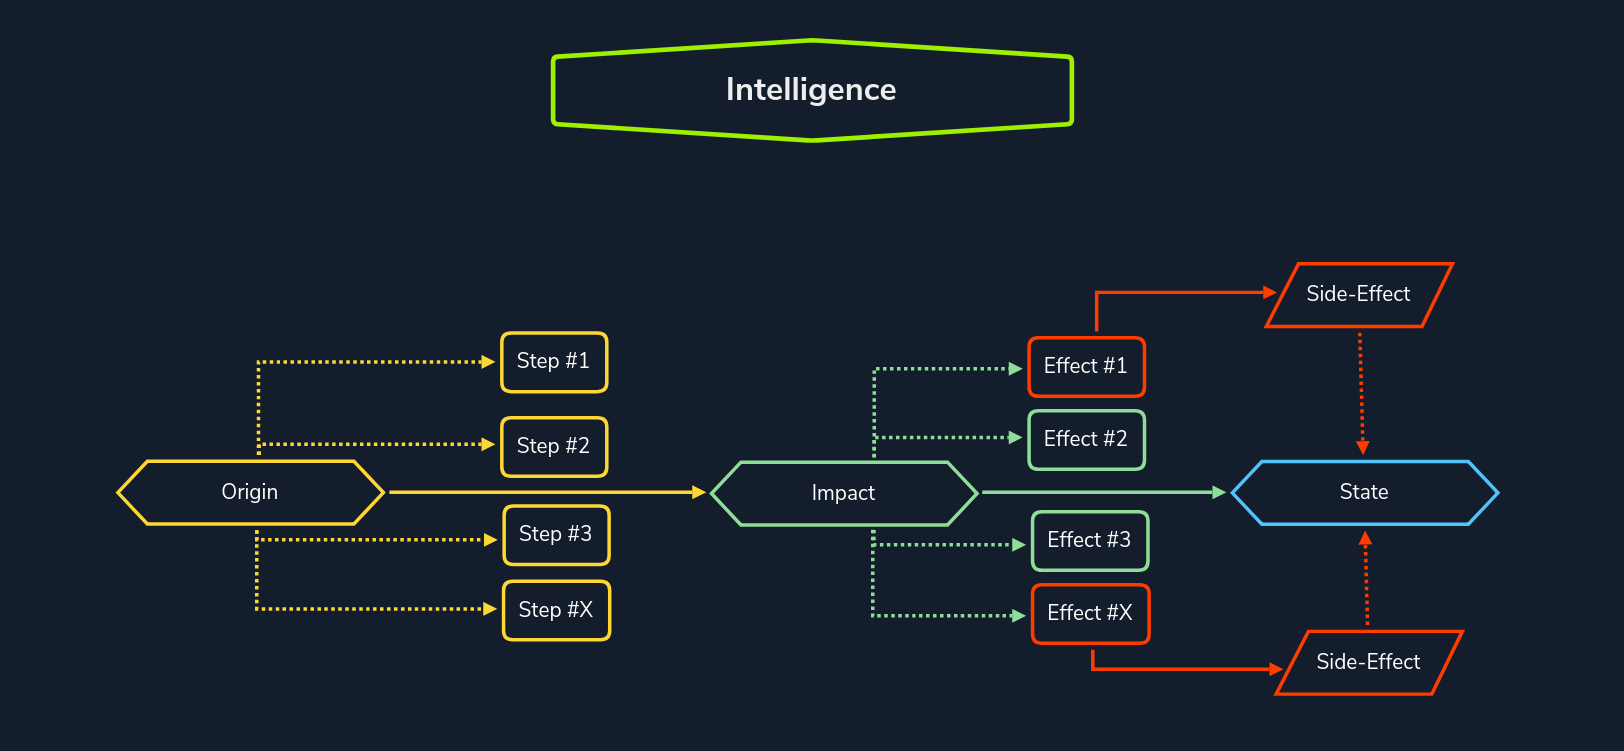
\includegraphics[width=\linewidth]{recon/osint/images/intelligence1.png}
  \caption{OSINT Intelligence}
  \label{fig:osint-intelligence}
\end{figure}

\subsubsection{Origin}
{\bf Each origin refers to an activity carried out in the past with the aim of
changing the future state through some particular impact.}

This means that each activity has a purpose and goal to be achieved. For us,
the necessary steps for this are essential. Therefore, we try to determine
which actions had to be taken to cause the desired impact to reach the current
state. Even if we do not know the state, we can use the steps to calculate its
impact and required actions to achieve the desired state.

\subsubsection{Impact}

To cause or provoke an impact, we need the combination of purpose or goal with
the corresponding action. The goal alone has no direct effect on the desired
state, just as little as an arbitrary action without a goal. Because with the
second, the result would lead to a random state. The steps that need to be
taken depend on the {\bf environment} and {\bf information}. Therefore, to
calculate the impact, we need information about the current state and the
environment in which our target is located. Accordingly, we gain insight into
the dependent factors by which we can calculate step-by-step which actions have
to be executed to achieve the desired state's corresponding impact.

\subsubsection{State}

A state is the result and functioning of different goals and the actions that
have been taken to achieve them. The achievement of a particular state always
automatically leads to {\bf side-effects}. These side-effects are unintended
impacts on the object and/or its environment.

Especially in information security, side-effects define exactly the
component/vulnerability we try to detect during our penetration tests. We can
say that no security-conscious administrator wants to make their company's
network vulnerable or put it at risk. The misconfigurations caused by those
side-effects of the actions to achieve the desired state and functionality are,
in most cases, unintentional. These are precisely the flaws that we as
penetration testers use to uncover these vulnerabilities in combination with
our objectives (simulation of an attacker) and the actions based on an example
(in a penetration test), which impact these can have on the company.

\subsubsection{Next Steps}

During our OSINT investigation, we only have information on the different
conditions for different periods. To understand the impact between two
different states and thus discover the potential side-effects, we need to
recreate the individual steps between impact and state as best as possible by
linking the information gathered.

As an example, we can take a simple software update. In simple terms, an update
is an improvement of the existing software and its version. Thus, the old
version would be the origin, and the new one would be the current state. The
developers had set themselves individual goals before developing a new version,
improving the service, or closing specific security vulnerabilities or bugs.
The individual steps represent the development process in which the code is
renewed, expanded, and improved. Each change (action) to the code has an impact
on the entire software. This can be new functions or improved performance.
However, this can lead to new errors and bugs, representing the side-effects we
want to discover.

Therefore, the art is to track these single steps and, in the best case, as
many as possible. To do this, we need to put ourselves in the administrator's
shoes as best we can. This is also the role of the feedback left by employees,
discovered during our investigation. This feedback gives us an impression of
the working atmosphere and its conditions. A lousy atmosphere leads to
dissatisfaction, demotivation, carelessness, and finally to mistakes that we
try to discover. Once we have found which side-effects have arisen or could
have arisen, we gain an accurate picture of how the software works and thus an
understanding of what actions we need to take to achieve our desired state of
the software.






\chapter{OSINT tools}
\url{https://osintfr.com/fr/outils/}

\url{https://info.signal-arnaques.com/bonnes-pratiques/outils-osint/}

\section{Sock puppet}
\subsection{introduction}
Simply put, a sock puppet is an alternative profile usually, a social media
profile, which you create intending to gather open-source information, with the
restriction that this profile will not link back directly to your original
account.

Sock puppets have two significant roles: utility and security:
\begin{itemize}
    \item Utility: Creating a specific social networking profile for the sake of collecting information makes logic from a utility perspective. Either you are aiming to befriend anyone on LinkedIn, seek to friend anyone on Facebook, or follow someone on their personal Instagram profile, you may want to make a more appealing profile to the individual or company you’re investigating. So, from a utility point, creating a new identity for the sake of your investigation is a no-brainer.
    \item Security: Sock puppets are also handy from a security perspective. Making up an alternative profile that does not explicitly link back to you is just neat OPSEC. If you are investigating an individual or organization, you likely do not want them to realize who you are or that you’re probing into something. During investigations, sock puppet offers anonymity as well as OPSEC to both the investigator and the victim.
\end{itemize}


Pre-questions of Sock Puppet

If you do a bit of pre-work, creating up your profile will be a lot simpler, and the result will be far more efficient. I would like you to think about anonymity and persistence.
\begin{itemize}
    \item Do you require complete anonymity on that profile? However, when I say anonymous, I am referring to the fact that a sock puppet does not usually lead back to you, but it might. You must make this profile in such a manner that it is anonymous, so that no matter how much a corporation investigates, they will most likely not be able to trace it to you.
    \item A persistent profile is simply a fictitious character you create to communicate with others on social networking sites. For days, months, or even seasons, you will be building contacts on LinkedIn, following personal Instagram profiles, or invading social networking sites, and that is a constant activity. You will need to do a great deal of research to establish this profile in such a manner that it will meet your objectives. Investigating publicly accessible assets is much effective with a persistent profile.
\end{itemize}



\subsection{How to Setup Sock Puppet Account?}

\subsection{Persona}
Create a character for the sock puppet profile. Prepare at the very least the
following:  

\begin{itemize}
    \item Name / Age / Gender: Create a character with a \href{https://www.fakenamegenerator.com/}{FakeNameGenerator} that meets your sockpuppet persona.
    \item image: To render an image, use
        \href{https://www.thispersondoesnotexist.com/}{This Person Does Not
        Exist}. Be sure to assess the picture carefully and choose one that
        does not have any apparent defects, as they always do. Use Photopea
        right in the browser if you need to modify an image.
\end{itemize}

\url{https://www.elfqrin.com/fakeid.php}

\subsubsection{Burner Phone}

Buy a burner phone that has been clean and is ready to use. It’s nearly
difficult to make a profile these days without getting a non-VOIP mobile
number. Purchase a low-cost mobile to use it as anonymously as necessary.

\subsubsection{SIM Card}

A new SIM card provides you with separate contact details. Mint Mobile’s 7-day
trial on Amazon is the cheapest SIM card. If you make a new profile, register
with a privacy.com  disguised credit/debit card, and get it delivered to an
Amazon locker, you can order it anonymously.

\subsubsection{Access Wi-Fi}

Do not access your own house or workplace Wi-Fi with an actual IP address. You
can’t choose a VPN because it will almost certainly stop you from making a
profile. Pick a good location like a library that is not directly beside your
home but is near enough.

\subsubsection{Email Account}

Create a primary email address. You can set up other email accounts afterward,
but you’ll want to start with a single main email account to which you will
configure everything. I propose creating a Google account and a
\href{https://protonmail.com/?ref=hackernoon.com}{Protonmail account} at the
very least. Both are useful at various periods.

\url{https://www.mail.com/}

\subsubsection{Setup 2FA}

Set up 2FA on all of your profiles. Where at all necessary, use a hardware
device like the YubiKey.

\subsubsection{VOIP Number}

Switch the contact information to the one you have more direct access to, such
as MySudo or Google Voice, once you’ve configured 2FA for all of the profiles.

\subsubsection{Steps to Configure Sock Puppet Accounts}

You have got all to make profiles on Facebook, Twitter, LinkedIn, Instagram, and other social media sites. Take time to set up each profile from beginning to end, storing all of the details in your password manager in the following order:
\begin{itemize}
    \item  Create the account (Use public Wi-Fi instead of a VPN with new contact details).
    \item  Once you create a profile, head straight to the security and privacy options.
    \item  Swap Mint mobile number with VOIP number.
    \item  Configure 2FA, ensure everything is in working order, wipe the mobile and ruin the SIM card.
\end{itemize}

\subsection{links}
\href{https://www.nortonlifelock.com/blogs/norton-labs/identifying-sockpuppet-accounts-social-media}{Identifying
Sockpuppet Accounts on Social Media Platforms}

\href{https://www.secjuice.com/the-art-of-the-sock-osint-humint/}{The Art Of
The Sock}

DeBot: Twitter Bot Detection via Warped Correlation

\href{https://medium.com/dark-roast-security/dark-side-116-sock-puppets-ed7a9bd5a556}{Dark
    Side 116: Sock Puppets. What if I told you not all fake social media
accounts are used maliciously?}

\href{https://osintcurio.us/2020/08/17/creating-research-accounts-for-osint-investigations/}{Creating
Research Accounts for OSINT Investigations}


\section{Burn phone}
\url{https://www.howtogeek.com/712588/what-is-a-burner-phone-and-when-should-you-use-one/}

\url{https://www.echosdunet.net/dossiers/telephone-jetable}

